%% 
%% Copyright 2007-2020 Elsevier Ltd
%% 
%% This file is part of the 'Elsarticle Bundle'.
%% ---------------------------------------------
%% 
%% It may be distributed under the conditions of the LaTeX Project Public
%% License, either version 1.2 of this license or (at your option) any
%% later version.  The latest version of this license is in
%%    http://www.latex-project.org/lppl.txt
%% and version 1.2 or later is part of all distributions of LaTeX
%% version 1999/12/01 or later.
%% 
%% The list of all files belonging to the 'Elsarticle Bundle' is
%% given in the file `manifest.txt'.
%% 

%% Template article for Elsevier's document class `elsarticle'
%% with numbered style bibliographic references
%% SP 2008/03/01
%%
%% 
%%
%% $Id: elsarticle-template-num.tex 190 2020-11-23 11:12:32Z rishi $
%%
%%
\documentclass[a4paper,12pt]{elsarticle}

%% Use the option review to obtain double line spacing
%% \documentclass[authoryear,preprint,review,12pt]{elsarticle}

%% Use the options 1p,twocolumn; 3p; 3p,twocolumn; 5p; or 5p,twocolumn
%% for a journal layout:
%% \documentclass[final,1p,times]{elsarticle}
%% \documentclass[final,1p,times,twocolumn]{elsarticle}
%% \documentclass[final,3p,times]{elsarticle}
%% \documentclass[final,3p,times,twocolumn]{elsarticle}
%% \documentclass[final,5p,times]{elsarticle}
%% \documentclass[final,5p,times,twocolumn]{elsarticle}

%% For including figures, graphicx.sty has been loaded in
%% elsarticle.cls. If you prefer to use the old commands
%% please give \usepackage{epsfig}

%% The amssymb package provides various useful mathematical symbols
\usepackage{amssymb}
\usepackage{appendix}
\usepackage{comment}
\usepackage{url}
\usepackage{tikz}
\usepackage{tabularx}
\usepackage[hscale=0.8,vscale=0.9]{geometry}
\usepackage[symbol]{footmisc}

\renewcommand{\deg}{\si{\degree}\xspace} % Use \deg easily, everywhere
\DeclareRobustCommand{\legendsquare}[1]{%
  \tikz[baseline=(a.south)]{\node[#1, inner sep=.8ex, outer sep=0] (a) {};}%
  }
\usepackage{colortbl}
\usepackage{graphicx}
\usetikzlibrary{shapes.geometric, arrows, fit}
\usetikzlibrary{arrows.meta}
\usetikzlibrary{automata,positioning}
\usetikzlibrary{shapes.multipart}
\usetikzlibrary{shapes.arrows,calc,positioning}
\definecolor{vent}{RGB}{255, 176, 0}
\definecolor{therm}{RGB}{220, 38, 127}
\definecolor{resp}{RGB}{100, 143, 255}
\definecolor{dyn}{RGB}{254, 97, 0}
\definecolor{TUgreen}{RGB}{108, 194, 74}
\definecolor{TUgreen_pastel}{RGB}{181, 225, 164}
\definecolor{TUblue}{RGB}{0,166,214}
\definecolor{TUblue_pastel}{RGB}{140,199,215}
\definecolor{TUyellow}{RGB}{255, 184, 28}
\definecolor{TUyellow_pastel}{RGB}{252, 216, 142}
\definecolor{TUred}{RGB}{165, 0, 52}
\definecolor{TUviolet}{RGB}{111, 29, 119}
\definecolor{TUorange}{RGB}{237, 104, 66}
\definecolor{TUteal}{RGB}{0,184,200}
\definecolor{TUmarine}{RGB}{0,118,194}
\definecolor{TUocean}{RGB}{0,155,119}
\usepackage{pgfgantt}
\usepackage{nicematrix}
\usepackage{floatrow}
\floatsetup[table]{capposition=top}
\usepackage{caption}
\captionsetup[table]{labelsep=period}
\captionsetup[figure]{labelsep=period}
\usepackage{comment}
\usepackage{tikz}
\usetikzlibrary{shapes.geometric, arrows}
\tikzstyle{startstop} = [rectangle, rounded corners, minimum width=5cm, minimum height=1cm,text centered, draw=black]
\tikzstyle{io} = [rectangle, minimum width=3cm, minimum height=1cm, text centered,text width=3cm, draw=black]
\tikzstyle{process} = [rectangle, minimum width=3cm, minimum height=1cm, text centered, text width=3cm, draw=black]
\tikzstyle{decision} = [diamond, minimum width=3cm, minimum height=1cm, text centered,text width=3cm, draw=black]
\tikzstyle{arrow} = [thick,->,>=stealth]
\usetikzlibrary{mindmap}
\usepackage{optidef}
\usepackage{siunitx}
\usepackage{longtable}
\setlength\parskip{\smallskipamount}
\DeclarePairedDelimiterXPP\BigOSI[2]%
  {\mathcal{O}}{(}{)}{}%
  {\SI{#1}{#2}}
\usepackage{scalefnt}
\usepackage{mathtools}
\usetikzlibrary{shapes.geometric, arrows, fit}
\usetikzlibrary{automata,positioning}
\usetikzlibrary{shapes.multipart}
\usetikzlibrary{shapes.arrows,calc,positioning}
\usepackage[hidelinks]{hyperref}
%% The amsthm package provides extended theorem environments
%% \usepackage{amsthm}

%% The lineno packages adds line numbers. Start line numbering with
%% \begin{linenumbers}, end it with \end{linenumbers}. Or switch it on
%% for the whole article with \linenumbers.
%% \usepackage{lineno}

\journal{Building and Environment}

\begin{document}

\begin{frontmatter}

%% Title, authors and addresses

%% use the tnoteref command within \title for footnotes;
%% use the tnotetext command for theassociated footnote;
%% use the fnref command within \author or \address for footnotes;
%% use the fntext command for theassociated footnote;
%% use the corref command within \author for corresponding author footnotes;
%% use the cortext command for theassociated footnote;
%% use the ead command for the email address,
%% and the form \ead[url] for the home page:
%% \title{Title\tnoteref{label1}}
%% \tnotetext[label1]{}
%% \author{Name\corref{cor1}\fnref{label2}}
%% \ead{email address}
%% \ead[url]{home page}
%% \fntext[label2]{}
%% \cortext[cor1]{}
%% \affiliation{organization={},
%%             addressline={},
%%             city={},
%%             postcode={},
%%             state={},
%%             country={}}
%% \fntext[label3]{}

\title{Quantifying airborne transmission in ventilated settings:\\ A review}

%% use optional labels to link authors explicitly to addresses:
%% \author[label1,label2]{}
%% \affiliation[label1]{organization={},
%%             addressline={},
%%             city={},
%%             postcode={},
%%             state={},
%%             country={}}
%%
%% \affiliation[label2]{organization={},
%%             addressline={},
%%             city={},
%%             postcode={},
%%             state={},
%%             country={}}

\author[inst1]{Arghyanir Giri \footnote[2]{\href{mailto:a.giri@tudelft.nl}{a.giri@tudelft.nl}, +31 641314917}}

\affiliation[inst1]{organization={Faculty of Architecture and the Built Environment, Delft University of Technology},%Department and Organization
            addressline={Julianalaan 134}, 
            city={Delft},
            postcode={2628BL}, 
            state={Zuid Holland},
            country={The Netherlands}}

\author[inst1]{Clara García-Sánchez}
\author[inst1]{Philomena M. Bluyssen}

%\affiliation[inst2]{organization={Department of Urbanism, Delft University of Technology},%Department and Organization
            %addressline={Julianalaan 134}, 
            %city={Delft},
            %postcode={2628BL}, 
            %state={Zuid Holland},
            %country={The Netherlands}}

\begin{abstract}
%% Text of abstract
As mandatory masking and social distancing measures decrease post-COVID-19, the risk of airborne pathogen transmission in crowded indoor spaces remains a significant public health concern. The pandemic highlighted the critical role of indoor air quality and ventilation in mitigating the spread of infectious diseases, underscoring the urgent need to improve our understanding and prediction of indoor airflow to minimize airborne transmission. In this review, studies on airborne transmission in indoor settings were systematically reviewed to identify research gaps and recommend changes in approach. The analysis is categorized into indoor airflow, droplet dynamics, and investigation methodologies. Findings reveal that almost 40\% of the reviewed literature does not specify the type of indoor setting, with only 3\% focusing on restaurant environments. Additionally, indoor air conditions are typically assumed to be constant, and respiratory activities are often limited to coughing and breathing. The review identifies the challenge of replicating the complex behaviour of respiratory aerosols in experiments and the computational expense of predicting turbulent indoor flows. Recommendations for future research include: i) focusing on social settings like restaurants, ii) considering varying air temperatures and humidity, iii) examining speech-related respiratory flows, and iv) employing visual and accurate tools to investigate particle-laden airflow. These insights aim to enhance public health guidelines and building designs to reduce the risk of airborne diseases.

\end{abstract}

\begin{comment}
%%Graphical abstract
\begin{graphicalabstract}

\includegraphics{grabs}
\end{graphicalabstract}

%%Research highlights
\begin{highlights}
\item Research highlight 1
\item Research highlight 2
\end{highlights}
\end{comment}

\begin{keyword}
%% keywords here, in the form: keyword \sep keyword
Airborne transmission \sep Ventilation \sep Multiphase fluid dynamics \sep Respiratory flows \sep Indoor Turbulence

\begin{comment}
  %% PACS codes here, in the form: \PACS code \sep code
\PACS 0000 \sep 1111
%% MSC codes here, in the form: \MSC code \sep code
%% or \MSC[2008] code \sep code (2000 is the default)
\MSC 0000 \sep 1111  
\end{comment}

\end{keyword}

\end{frontmatter}

%% \linenumbers

%% main text
\section{Introduction}
\label{sec:sample1}

Since the onset of the COVID-19 pandemic, over 600 million people have been infected by the SARS-CoV-2 virus, and over 6 million people have lost their lives as of last December 2023 \cite{world2023therapeutics}. A boom in scientific research focused on containing, limiting, and mitigating the spread of the SARS-CoV-2 virus has been observed since the outbreak began in Wuhan in early 2020 \cite{morawska2020can,morawska2020time}. Numerous scientists made a critical suggestion that the concerned virus is airborne-spread \cite{zhang2020identifying,bazant2021guideline,morawska2020airborne}. Fortunately, the outbreak was managed with the help of public health guidelines on mandating masks, contact tracing, and social distancing. However, there was some resistance and debate on its transmission route. It was initially believed to be a droplet-spread disease that limited the transmission routes to coughing, sneezing, and direct inhalation from contaminated surfaces \citep{chagla2021re}. It took some time for health advice to catch up with the scientific findings as WHO took almost two years to include 'long-range airborne transmission' in their official statements \cite{lewis2022took}.

One of the steps taken to curb the spread of SARS-CoV-2 was the use of sufficient ventilation as it has proven to be an effective measure to curb the spread of viruses \cite{ren2021numerical}, pathogens \cite{berrouk2010experimental} or contaminants \cite{li2020investigating}. Many studies have suggested that long-range transmission occurred inside poorly ventilated settings in the initial stages of the COVID-19 pandemic \cite{morawska2020can,li2021probable, liu2021simulation}. As most public health guidelines have been eased now and everyone is leading their usual lives, studying the airborne transmission of pathogens at this point is not an analysis of what happened in the past but a preparation for the next pandemic ahead of us. Therefore, the role of indoor ventilation in minimizing infection risk cannot be understated in the current scenario.

Previously, airborne transmission in an indoor environment has been looked at from epidemiological, biological, physical, and computer modelling perspectives \cite{argyropoulos2023airborne}. The studies focused on modelling highlighted common limitations like averaging the effects of turbulence \cite{mirzaie2021covid,dbouk2020respiratory}, neglecting the impact of small-scale eddies, and using tracer gases to understand aerosol dynamics that fail to capture properties like volatility and deposition on surfaces \cite{rayegan2022review, zhao2022airborne}. The importance of ventilation design is illustrated by various reviews like \cite{luongo2016role}, \cite{hobeika2023assessing} \& \cite{thornton2022impact}, which show how good ventilation design mitigates transmission. At the same time, \citet{correia2020airborne} suggests how inadequate ventilation can become a reason for long-range transmission.

While researchers unanimously agree that indoor environments require sufficient ventilation, increasing the room's ventilation rate will not reduce the risk of exposure to pathogen-laden droplets. Some more nuances in ventilating a room still need to be addressed. Although a high ventilation rate helps with the removal of pathogens in a room \cite{guo2022visualization, ho2021modeling}, it does not necessarily reduce the droplet concentration near an occupant \cite{arpino2023cfd}. Additionally, recirculating the same air within the room without proper filtering or treatment is another flaw in current ventilation systems \cite{li2021probable}. There is a pressing need to develop methods to predict and quantify the airborne transmission potential of viruses based on model studies, experiments, and outbreak research. The present study is a systematic review of research on expelled respiratory droplets in a ventilated setting and the associated risk of infection. This review aims to understand different ventilation regimes and their effect on airflow and droplets to minimize airborne transmission of pathogens.

\section{Methods}

For the review, Web of Science, Scopus, and PubMed were chosen as the databases for searching relevant literature. This review covers five broad topics: (a) transmission of the pathogen, (b) ventilation regime, (c) investigation approach, (d) setting, and (e) risk analysis. Keywords were chosen under each broad topic to identify relevant literature in the web databases as shown in Table \ref{tab:keys}. Boolean operators `AND'/'OR' were used to combine the search terms and construct a query. The Boolean operator `OR' was used to combine the keywords of each broad topic to form a search query for the corresponding category. The search query from each category was combined to create a final search query using the `AND' boolean operator. This search query identified articles through the abstract, title, and keywords across all the databases.

The term ``SARS-CoV-2 Transmission" was used under the family of keywords even though this study does not focus only on "SARS-CoV-2" because of the large number of articles that solely refer to the virus in the past two to three years. Additionally, under the category of `Ventilation', the truncated form ``Ventilat*" was used to identify articles that have used it in a different form, along with terms like ``Air cleaning" and ``Filtration". The latter two were included because some settings used air purifiers instead of conventional ventilation systems. More truncated forms like ``Model*", ``Simulat*", and ``Experiment*" were used to cover every ending of the root word under the `Investigation' category. Search terms like ``Machine learning" and "Deep learning" were included to look for articles using ML or DL to accelerate CFD.

{\renewcommand{\arraystretch}{1.1}
\begin{table}
\footnotesize
\captionsetup{font=normalsize}
    \begin{tabularx}{\textwidth}{|p{2.5cm}|X|p{2.5cm}|X|X|}
    \hline
    \multicolumn{5}{|c|}{\textbf{Broad concepts and Keywords}} \\
    \hline
    \textbf{Transmission} & \textbf{Ventilation} & \textbf{Investigation} & \textbf{Setting} & \textbf{Risk Analysis}\\
    \hline
    Airborne Transmission & Ventilat* & Model* & Indoor setting & Risk Assessment \\
    Aerosol Transmission & Air cleaning & Simulat* & Environment & Infection probability\\
    Indoor Transmission & HVAC & Experiment* & Confined spaces & Exposure \\         
    SARS-CoV-2 Transmission & Air change  & CFD & Office  & Wells-Riley\\        
    Indoor contamination & Filtration & Measurement & Restaurant & Dose-response\\        
    Environmental Transmission & Air distribution & Validation & Classroom & \\  
    Airborne route &  & Estimation & Hospital & \\
     &  & Machine Learning &  & \\
    &  & Deep Learning &  & \\
    \hline
    \end{tabularx}
    \caption{Broad concepts and keywords to construct the search query.}
    \label{tab:keys}
\end{table}
}

A total of 195 articles were found from Scopus, 258 from Web of Science, and 159 from PubMed. The duplicate articles were merged to obtain 385 unique papers from the databases. The initial screening of articles was conducted by reading titles and abstracts to classify them into different categories. Review papers were segregated from the articles for further screening for relevant studies. After separating the 38 review articles, the remaining 347 papers were screened for relevance to pathogen transmission in a ventilated indoor environment. Models based solely on theoretical reasoning, papers dealing with building-scale aerodynamics, papers not mentioning ventilation, purely epidemiological studies, and non-English and non-accessible papers were excluded. After excluding 130 papers that did not meet the first criteria, 218 papers that theoretically, experimentally, or computationally investigated airborne transmission of pathogens remained.

Papers including numerical simulations that were either paired with or validated against experimental studies were given preference, thus excluding purely qualitative studies, purely measurement-based studies, Reynolds Averaged Navier-Stokes (RANS) simulations that were not validated or were validated against theoretical models, and studies that focused on contaminants that were not droplet-based. An exception was made for some Large Eddy Simulations (LES) or Direct Numerical Simulations (DNS) investigating the spread of pathogens via aerosol droplets but not modelling ventilation. Their inclusion is essential as they are state-of-the-art in flow simulations for airborne transmission in ventilated settings. After the initial screening, 50 such research papers were selected for review.

The segregated 38 review articles were screened further for relevance, of which 13 papers reviewed articles on airborne transmission, approaches of research, and ventilation methods. There were 2046 references in the selected review papers, which were subjected to the same exclusion criteria as the initial screening. After screening the review papers, 26 additional research papers were found. The 26 research papers included five studies that used DNS and ten studies that used LES. The final set of articles comprises 76 research papers thoroughly reviewed and analyzed in the following sections. The review process is summarized in figure \ref{fig:flowchart}.

\begin{figure}
    \centering
    \tikzstyle{io} = [rectangle, minimum width=3cm, minimum height=1cm, text centered,text width=3cm, draw=black]
\tikzstyle{process} = [rectangle, minimum width=3cm, minimum height=1cm, text centered, text width=5cm, draw=black]
\tikzstyle{decision} = [diamond, minimum width=3cm, minimum height=1cm, text centered,text width=3cm, draw=black]
\tikzstyle{arrow} = [thick,->,>=stealth]
\tikzstyle{myfit1} = [draw,solid,black, inner xsep=25pt, inner ysep=25pt, rounded corners=5pt]
\tikzstyle{myfit3} = [draw,solid,black, inner xsep=10pt, inner ysep=20pt, rounded corners=5pt]
\tikzstyle{myfit4} = [draw,solid,black, inner xsep=10pt, inner ysep=10pt, rounded corners=5pt]
\tikzstyle{myfit2} = [draw,dashed,black, inner xsep=10pt, inner ysep=15pt, rounded corners=5pt]
\tikzstyle{mytitle1} = [draw,solid,black, fill=gray!50, inner sep=5pt]
\tikzstyle{mytitle2} = [draw,solid,black, fill=gray!50, inner sep=3pt]
\resizebox{\textwidth}{!}{\begin{tikzpicture}[thick,scale=0.6,node distance=2cm]
\node (start) [startstop] {\textbf{Airborne transmission in ventilated settings}};
\node (topic1) [io,below of=start,xshift=-7cm,yshift=-0.5cm] {\textbf{Transmission}\\7 keywords combined by OR};
\node (topic2) [io,below of=start,xshift=-3.5cm,yshift=-0.5cm] {\textbf{Ventilation}\\6 keywords combined by OR};
\node (topic3) [io,below of=start,yshift=-0.5cm] {\textbf{Investigation}\\9 keywords combined by OR};
\node (topic4) [io,below of=start,xshift=3.5cm,yshift=-0.5cm] {\textbf{Setting}\\7 keywords combined by OR};
\node (topic5) [io,below of=start,xshift=7cm,yshift=-0.5cm] {\textbf{Risk analysis}\\5 keywords combined by OR};
\node (quer) [io, below of=topic3,yshift=-0.5cm] {Final search query\\combined by AND};
\node (in0) [io, below of=quer,xshift=-3.5cm, yshift=-2cm] {Papers in Scopus\\(n = 195)};
\node (in1) [io, below of=quer,yshift=-2cm] {Papers in WoS\\(n = 258)};
\node (in15) [io,below of=quer,xshift=3.5cm,yshift=-2cm] {Papers in PubMed\\(n = 159)};
\node (in2) [io, below of=in1,yshift=-0.5cm] {Papers after merging duplicates\\(n = 385)};
\node (in3) [io, below of=in2,yshift=-0.5cm] {Non-review articles for screening\\(n = 347)};
\node (in4) [io, below of=in3,yshift=-0.5cm] {Relevant studies\\(n = 218)};
\node (in5) [io, right of=in2,xshift=2.5cm] {Review papers\\(n = 38)};
\node (in6) [io, below of=in4,yshift=-1cm] {Core papers after initial screening\\(n = 50)};
\node (in8) [io, below of=in5,] {Relevant reviews\\(n = 13)};
\node (in10) [io, below of=in8,yshift=-4cm] {Papers from reviews\\(n = 26)};
\node (ex1) [process,left of=in3, xshift = -4cm,yshift=0.8cm] {Excluded studies (n = 130)\\- theoretical models\\- building-scale studies\\- no discussion on ventilation\\- purely epidemiological studies\\- non English papers \\- not accessible};
\node (ex2) [process,left of=in4, xshift = -4cm,yshift = -1.8cm] {Excluded studies (n = 168)\\- unvalidated RANS\\- qualitative studies\\- purely measurement based\\- simulations validated against theoretical models\\- non-droplet contaminant};
\node (ex3) [io, right of=in8,xshift=2cm, yshift=-3.2cm] {Excluded\\references\\(n = 2046)\\-duplicates\\-unvalidated RANS\\-no droplets\\-no ventilation};
\node (cl1) [io, below of=in6,xshift=-4.5cm, yshift=-2cm] {Indoor airflow};
\node (cl2) [io, below of=in6, yshift=-2cm] {Droplet dynamics};
\node (cl3) [io, below of=in6,xshift=4.5cm, yshift=-2cm] {Investigation approaches};
\node (end) [startstop, below of=cl2, yshift=-1cm] {Discussion and Conclusions};
 
\draw [arrow] (start) -- node[anchor=west] {} (topic3);
\draw [arrow] (start) -| node[anchor=east] {} (topic1);
\draw [arrow] (start.189) -| node[anchor=east] {} (topic2.north);
\draw [arrow] (start.351) -| node[anchor=east] {} (topic4.north);
\draw [arrow] (start) -| node[anchor=west] {} (topic5);
\draw [arrow] (topic1) |- node[anchor=west] {} ([yshift=0.3cm]quer.west);
\draw [arrow] (topic2) |- node[anchor=east] {} ([yshift=0.3cm]quer.west);
\draw [arrow] (topic3) -- node[anchor=west] {} (quer);
\draw [arrow] (topic4) |- node[anchor=east] {} ([yshift=0.3cm]quer.east);
\draw [arrow] (topic5) |- node[anchor=west] {} ([yshift=0.3cm]quer.east);
\draw [arrow] (quer) -- node[anchor=west] {} (in1);
\draw [arrow] (quer) -| node[anchor=east] {} (in0);
\draw [arrow] (quer) -| node[anchor=west] {} (in15);
\draw [arrow] (in1) -- node[anchor=east] {} (in2);
\draw [arrow] (in0.270) -| node[anchor=east] {} ([xshift=-0.3cm]in2.north);
\draw [arrow] (in15.270) -| node[anchor=east] {} ([xshift=0.3cm]in2.north);
\draw [arrow] (in3) |- node[anchor=east] {} ([yshift=-3.6cm]ex1.east);
\draw [arrow] (in4) |- node[anchor=east] {} ([yshift=0.9cm]ex2.east);
\draw [arrow] (in8) |- node[anchor=east] {} (ex3);
\draw [arrow] (in2) -- node[anchor=west] {} (in3);
\draw [arrow] (in2) -- node[anchor=west] {} (in5);
\draw [arrow] (in3) -- node[anchor=west] {} (in4);
\draw [arrow] (in4) -- node[anchor=west] {} (in6);
\draw [arrow] (in5) -- node[anchor=west] {} (in8);
\draw [arrow] (in8) -- node[anchor=east] {} (in10); 


\node[fit=(topic1)(topic2)(topic3)(topic4)(topic5)(quer),myfit3] (strats) {};
\node[mytitle2] at ([xshift=-7cm]strats.south) {Search strategy};

\node[fit=(in0)(in1)(in15)(in2)(in3)(in4)(in5)(in6)(in8)(in10)(ex1)(ex2)(ex3),myfit3] (screening) {};
\node[mytitle2] at ([xshift=-7cm]screening.south) {Screening};


\node[fit=(cl1)(cl2)(cl3),myfit1] (analysis) {};
\node[mytitle2] at ([xshift=-7cm]analysis.south) {Analysis};
\draw[arrow](analysis) -- node[anchor=east] {} (end);

\node[fit=(in6)(in10),myfit4] (final) {};
\node[mytitle2] at (final.north) {Final set of papers};
\draw[arrow] ([xshift=-3.75cm]final.south) -- (analysis.north);


\end{tikzpicture}}
    \caption{The review process.}
    \label{fig:flowchart}
\end{figure}

\section{Outcome of review}

The review summarises studies on common airflow patterns in different ventilated settings, droplet physics in respiratory aerosols for indoor conditions, and experimental and simulation studies to mimic airborne transmission scenarios.

\subsection{Airflow in indoor environments}

Airborne transmission in an indoor environment calls for discussing airflow patterns, which are the bulk carriers of pathogen-laden aerosols. The indoor airflow has multiple components and differs according to the setting, air conditions, and occupancy. Indoor airflow mainly constitutes ventilation flow, flow due to temperature differences, and respiratory flows. Every setting has a unique configuration of occupants, obstructions and ventilation, making their interaction with different respiratory activities vary. The overlap between different sources of airflow inside various indoor environments is illustrated through Table \ref{tab:mat}, qualitatively highlighting the mixing potential of the flows.

Some standard occupant configurations and ventilation regimes were found in the review, of which three were selected. The selected occupant configurations and ventilation regimes are represented in a matrix illustrating the variation among the nine scenarios. The scenarios are visualised as simplified schematics roughly adapted from the previous research with different sources of airflow illustrated with different colours. Occupant configuration 1 is where the occupants are facing each other, and occupant configuration 2 is where the occupants are facing the same direction. Occupant configuration 3 is specific to a healthcare setting where one occupant is lying, and another is standing beside the bed.

The first occupant configuration is observed in hospitals \cite{zhou2021experimental}, offices \cite{li2023numerical}, and restaurants \cite{oksanen2022combining} where the two occupants are sitting facing each other, across a table as shown in the schematics. For this occupant configuration, the respiratory flows (shown in blue) collide head-on and spread axially depending on the offset height and laterally \cite{giri2022colliding, singhal2022virus} while the thermal flows (in red) rise upward with intensity depending on the temperature difference between the surface of the occupant and the air temperature \cite{zhang2019distribution}. The second occupant configuration is observed in classrooms \cite{qin2023transmission}, offices \cite{he2011cfd}, and modes of transport \cite{yan2021transmission,ho2021modeling} where the occupants are facing in the same direction. The respiratory flows in this configuration interact directly with the thermal flow \cite{ou2022insufficient}. The third configuration of occupants is unique to hospitals and healthcare settings where one or more occupants are lying and standing \cite{villafruela2019assessment, lu2020reducing}. The lying occupants are patients, while the standing are healthcare workers or visitors. In this case, the respiratory flow is parallel to the thermal flow, which results in a net upward flow. The surface area of the lying occupant is greater than that of a sitting occupant, resulting in laterally spread thermal plumes \cite{feng2020influence}.

In Table \ref{tab:mat}, Ventilation Regime 1 is mixing ventilation, Ventilation Regime 2 is displacement ventilation, and Ventilation Regime 3 is stratum and cross ventilation. Different overlaps between the three sources of airflow (differentiated by colour) are observed with the three different ventilation regimes. The schematics include directions for the ventilation airflow using arrows at the supply and exhaust. In Ventilation Regime 1, the direction of the flow is shown downwards, but the flow is not directly downwards; it is tangential to the ceiling surface. In the schematics, the respiratory flow originates from the mouth of the occupants, and thermal flow is upwards while originating from the occupant's body. 

\begin{table}[h!]
\captionsetup{font=normalsize}
    \footnotesize
    \centering
    \begin{tabular}{|m{2.5cm}|m{4cm}|m{4cm}|m{4cm}|}
    \hline
     & \textbf{Ventilation regime 1} & \textbf{Ventilation regime 2} & \textbf{Ventilation regime 3} \\
    \hline
    \textbf{Occupant Configuration 1} & 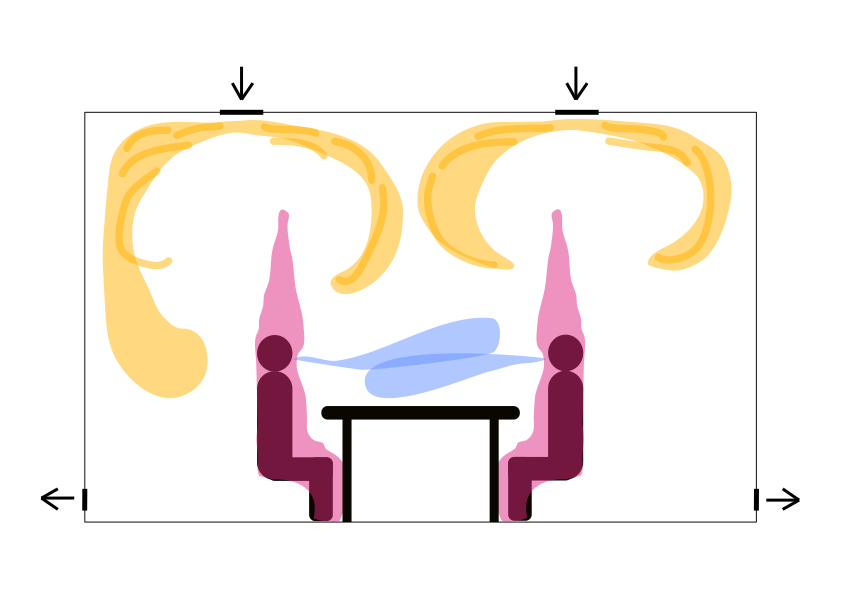
\includegraphics[clip,trim={0 2cm 0 2cm},width=0.25\textwidth]{Airflow/mat1.jpeg}& 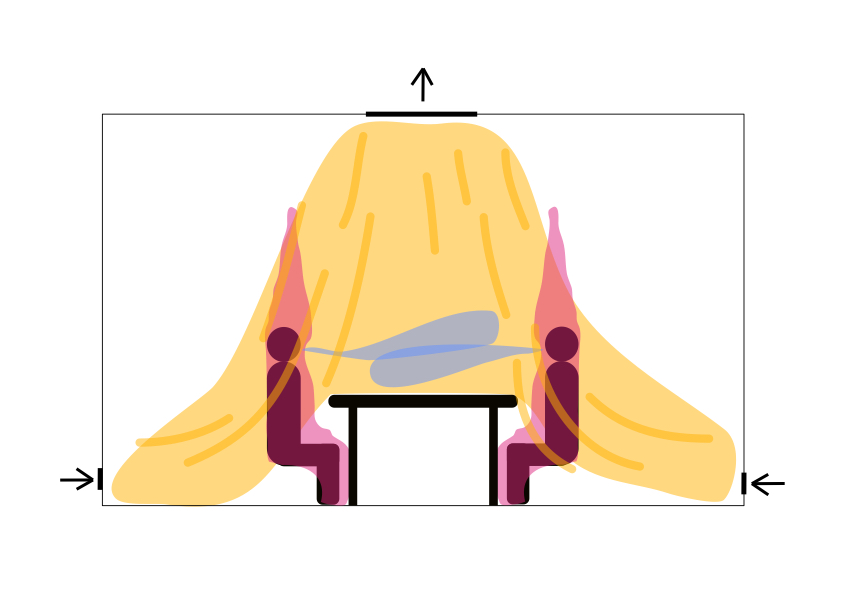
\includegraphics[clip,trim={0 2cm 0 2cm},width=0.25\textwidth]{Airflow/mat4.jpeg}& 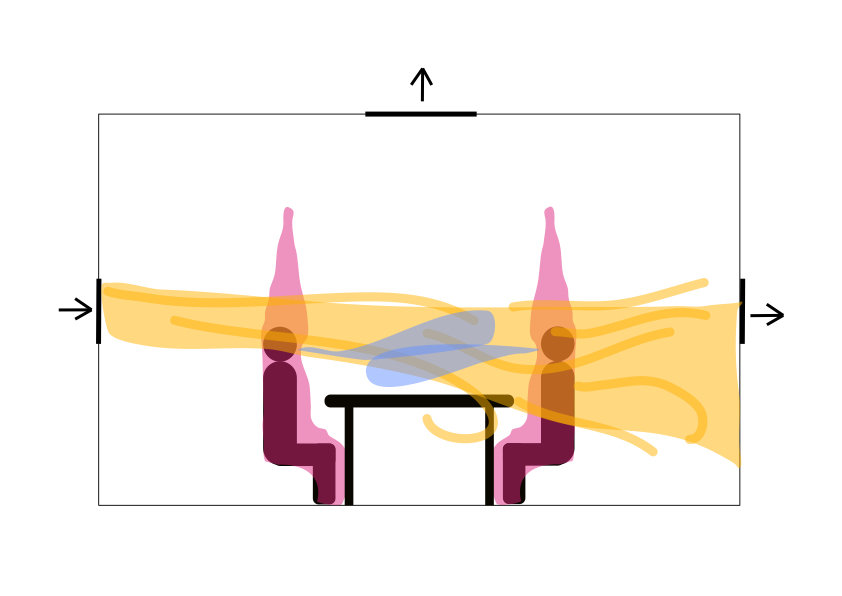
\includegraphics[clip,trim={0 2cm 0 2cm},width=0.25\textwidth]{Airflow/mat7.jpeg} \\
    \hline
    \textbf{References} & \cite{li2020investigating,zhou2021experimental,pan2022boundary,pan2023predicting,li2022airborne} & \cite{deng2021control,zhou2021experimental,wu2023numerical} & \cite{pendar2020numerical,feng2020influence} \\
    \hline
    \textbf{Occupant Configuration 2} &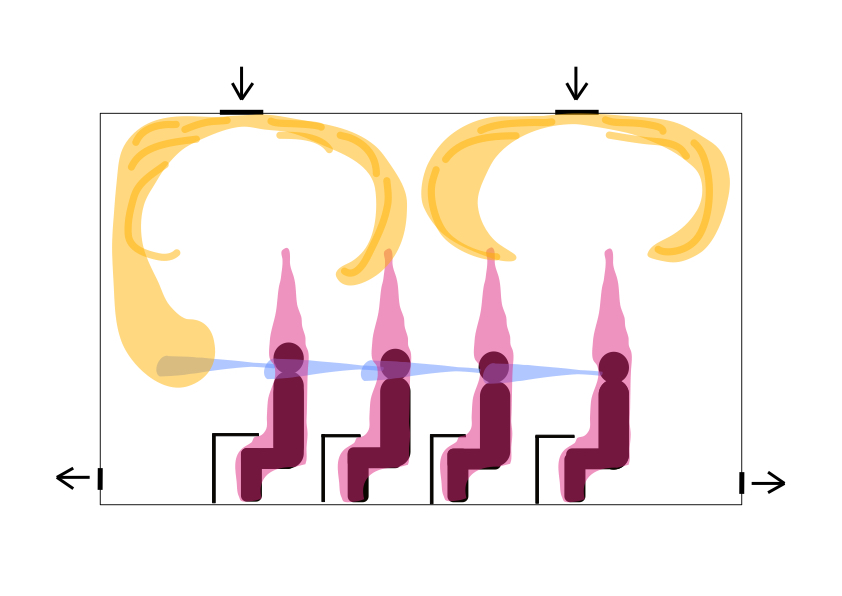
\includegraphics[clip,trim={0 2cm 0 2cm},width=0.25\textwidth]{Airflow/mat2.jpeg}& 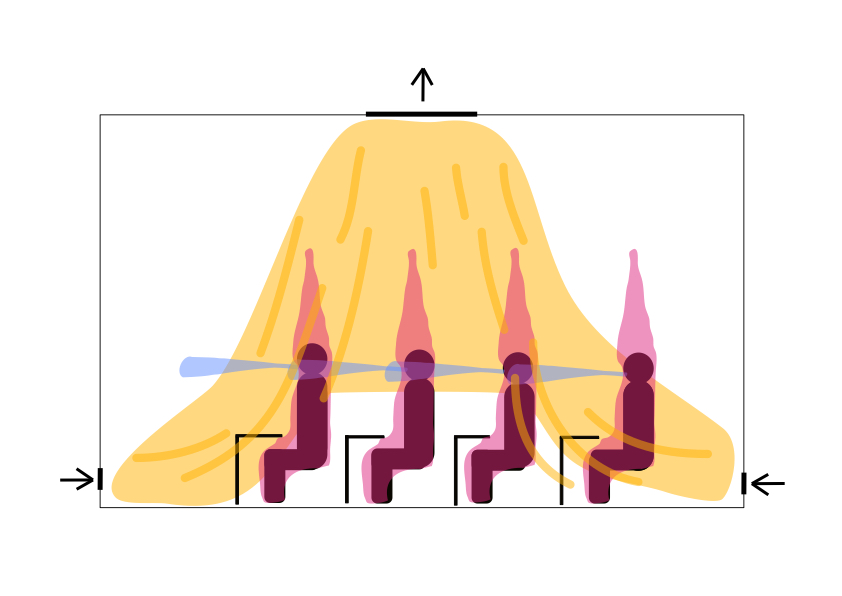
\includegraphics[clip,trim={0 2cm 0 2cm},width=0.25\textwidth]{Airflow/mat5.jpeg}& 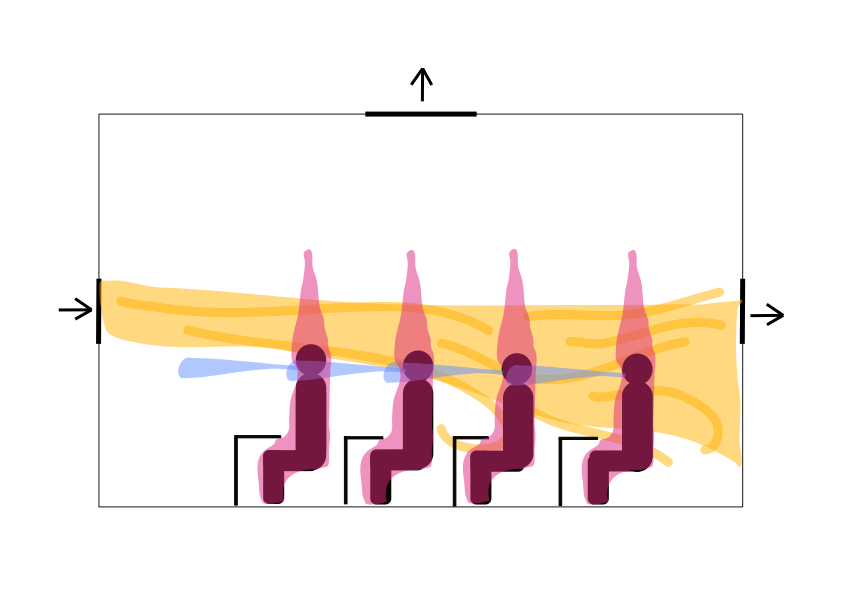
\includegraphics[clip,trim={0 2cm 0 2cm},width=0.25\textwidth]{Airflow/mat8.jpeg} \\
    \hline
    \textbf{References} & \cite{he2011cfd,yan2021transmission,mirzaie2021covid,li2021effects,shao2021risk,qin2023transmission,xu2023cfd} & \cite{he2011cfd,lu2022ventilation,jain2023numerical} & \cite{ho2021modeling,duill2021impact,ren2022practical,lu2022ventilation} \\
    \hline
    \textbf{Occupant Configuration 3} &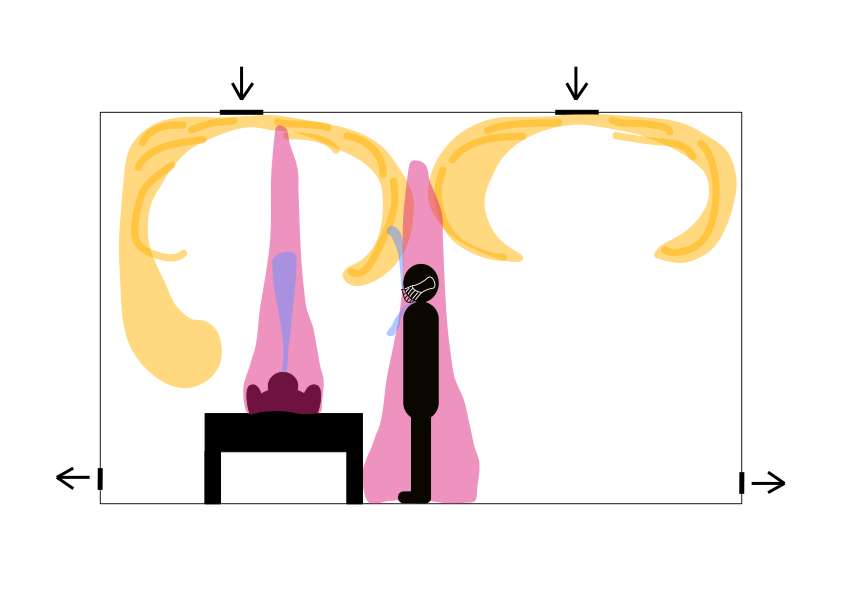
\includegraphics[clip,trim={0 2cm 0 2cm},width=0.25\textwidth]{Airflow/mat3.jpeg}& 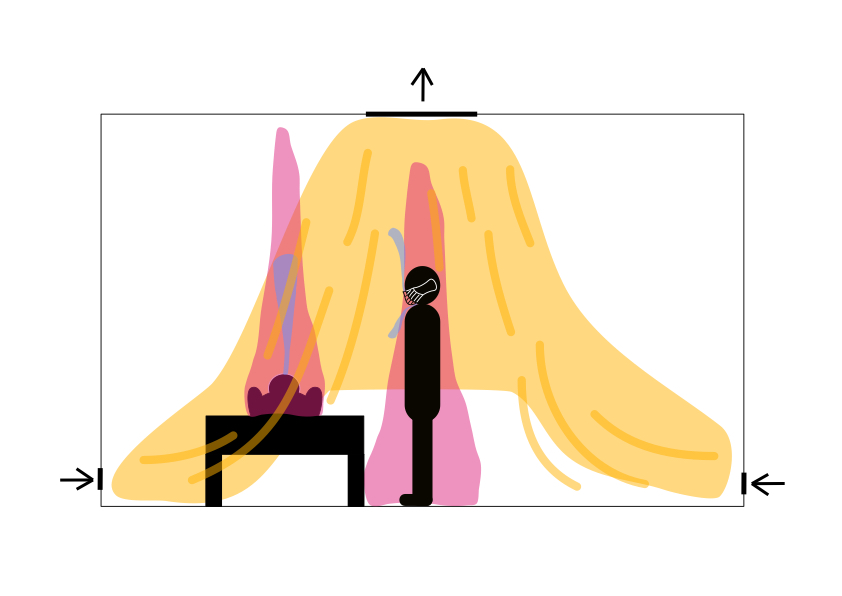
\includegraphics[clip,trim={0 2cm 0 2cm},width=0.25\textwidth]{Airflow/mat6.jpeg}& 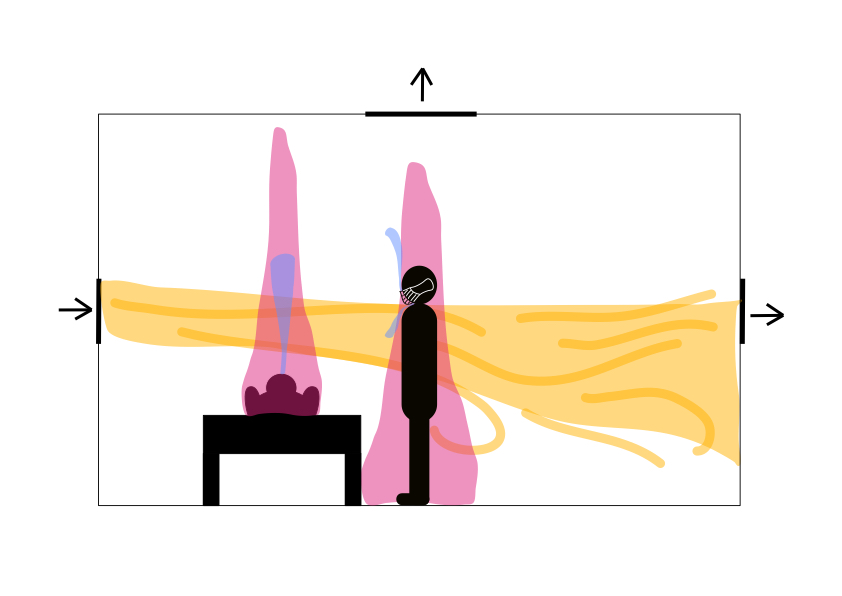
\includegraphics[clip,trim={0 2cm 0 2cm},width=0.25\textwidth]{Airflow/mat9.jpeg} \\
    \hline
    \textbf{References} & \cite{hang2014influence,romano2015numerical,liu2020full,lu2020reducing,zhou2021experimental,guo2022visualization,liu2023estimating} & \cite{zhou2021experimental,villafruela2019assessment,lu2020reducing} & \cite{jiang2009investigating,lu2020reducing} \\
    \hline
    \end{tabular}
    \caption{Schematics for indoor airflow matrix with three common occupant configurations and three common ventilation regimes.}
    \label{tab:mat}
    \vspace{0.5cm}
    \normalsize
        NOTE: The airflow is differentiated into three types with colours as follows:\\ \legendsquare{fill=resp} Respiratory flow \legendsquare{fill=vent} Ventilation flow \legendsquare{fill=therm} Thermal flow 
\end{table}

    
\subsection{Droplet dynamics}

Pathogens are ejected via respiratory activity and transmitted from an infected individual to a susceptible one through direct/indirect airborne or fomite transmission \cite{leung2021transmissibility}. In every transmission route, pathogens exist in the form of aerosols, which can evaporate, condense, merge, and deposit, making simulating their behaviour complicated \cite{rosti2020fluid,zhou2021dynamical}. The air conditions, the type of respiratory activity, and the droplet's size significantly impact their physical behaviour and potential to carry pathogens across space.

Air temperature and relative humidity are two primary parameters describing air conditions in a room. The room's air temperature mainly affects the intensity of thermal currents from the occupants and, consequently, the propagation of respiratory droplets \cite{feng2020study}. Relative humidity mainly affects how long the droplet is suspended in the air, which affects the evolution of the droplet over time. Lower air temperatures result in higher buoyancy effects on the exhaled droplets, which lead to their accumulation near the ceiling \cite{zhang2019distribution}. Whereas high relative humidity protects the expelled respiratory droplets from evaporation \cite{chong2021extended}. The droplet plume schematics in the first two columns of Table \ref{tab:mat2} show the effect on droplet dynamics for different combinations of air conditions.

Humans shed droplets during respiratory activities like sneezing, coughing and speech \cite{stadnytskyi2021breathing}. These droplets often differ in velocity, size, and number. The droplets during a cough or sneeze are expelled at high velocities, thus reaching large distances away from the mouth in contrast to droplets expelled during speaking and breathing \cite{pendar2020numerical,zhang2019distribution}. Cough or sneeze droplets are more prominent in diameter (10-100 $\mu$m), while breathing produces smaller droplets ($\approx$1$\mu$m) \cite{shao2021risk}. On the other hand, speech sheds droplets of sizes ranging from 1$\mu$m to 1mm, where the bigger droplets settle down because of gravity while smaller ones follow the airflow \cite{tan2021experimental}. Time scales for sneezing and coughing are relatively small ($\approx$1s) compared to speech or breathing, where the activity can last longer ($\approx$1min). Moreover, the number of droplets produced is lower for coughing (1-1000$s^{-1}$) than speaking, which produces an order of magnitude higher number of droplets (1-10000$s^{-1}$) \cite{giri2022colliding}. Furthermore, the production of droplets is higher if the occupant speaks loudly or makes plosive sounds \cite{abkarian2020speech}. The second column in Table \ref{tab:mat2} shows the droplet plume schematics for the four different respiratory activities discussed above with different-sized droplets differentiated with colour.

\begin{table}[h!]
\captionsetup{font=normalsize}
    \footnotesize
    \centering
    \begin{tabular}{|m{2.5cm}|m{4cm}||m{2.5cm}|m{4cm}|}
    \hline
    \textbf{Air conditions} & \textbf{Schematic} & \textbf{Respiratory activity} & \textbf{Schematic} \\
    \hline
    Low air temperature \& Low humidity & 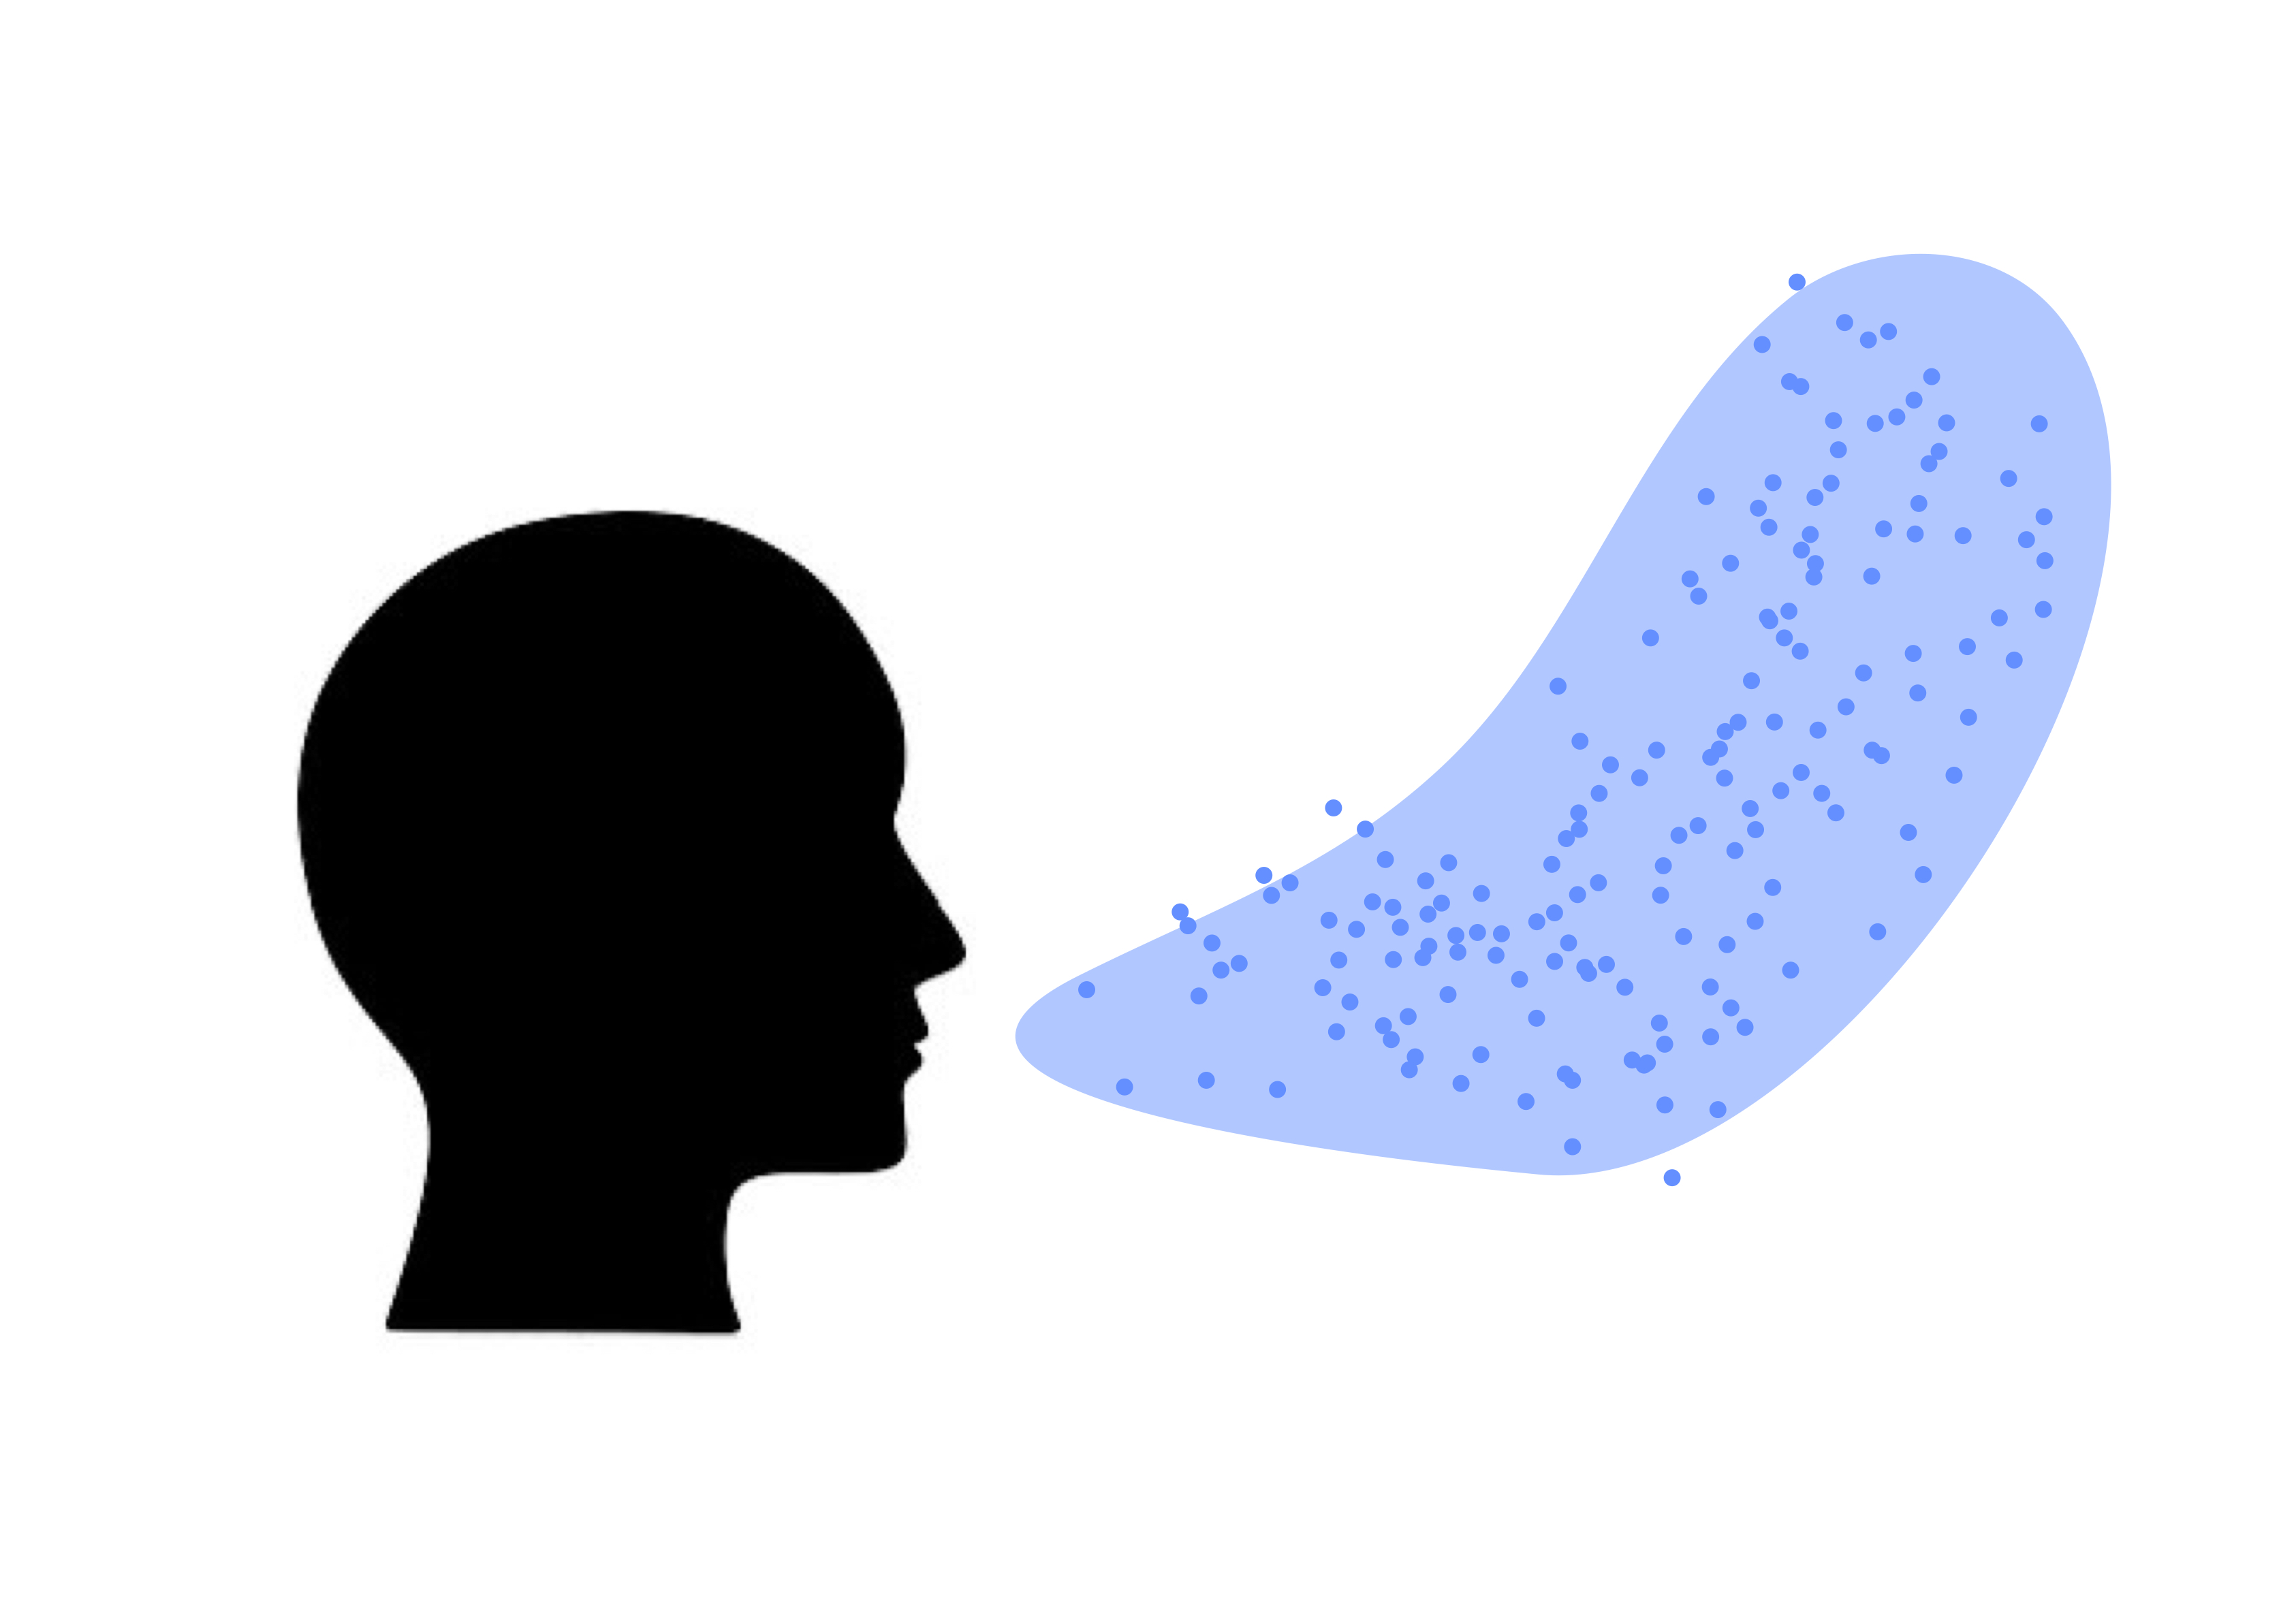
\includegraphics[clip,trim={0 2cm 0 2cm},width=0.25\textwidth]{Droplets/dropmat1.jpeg}& Coughing & 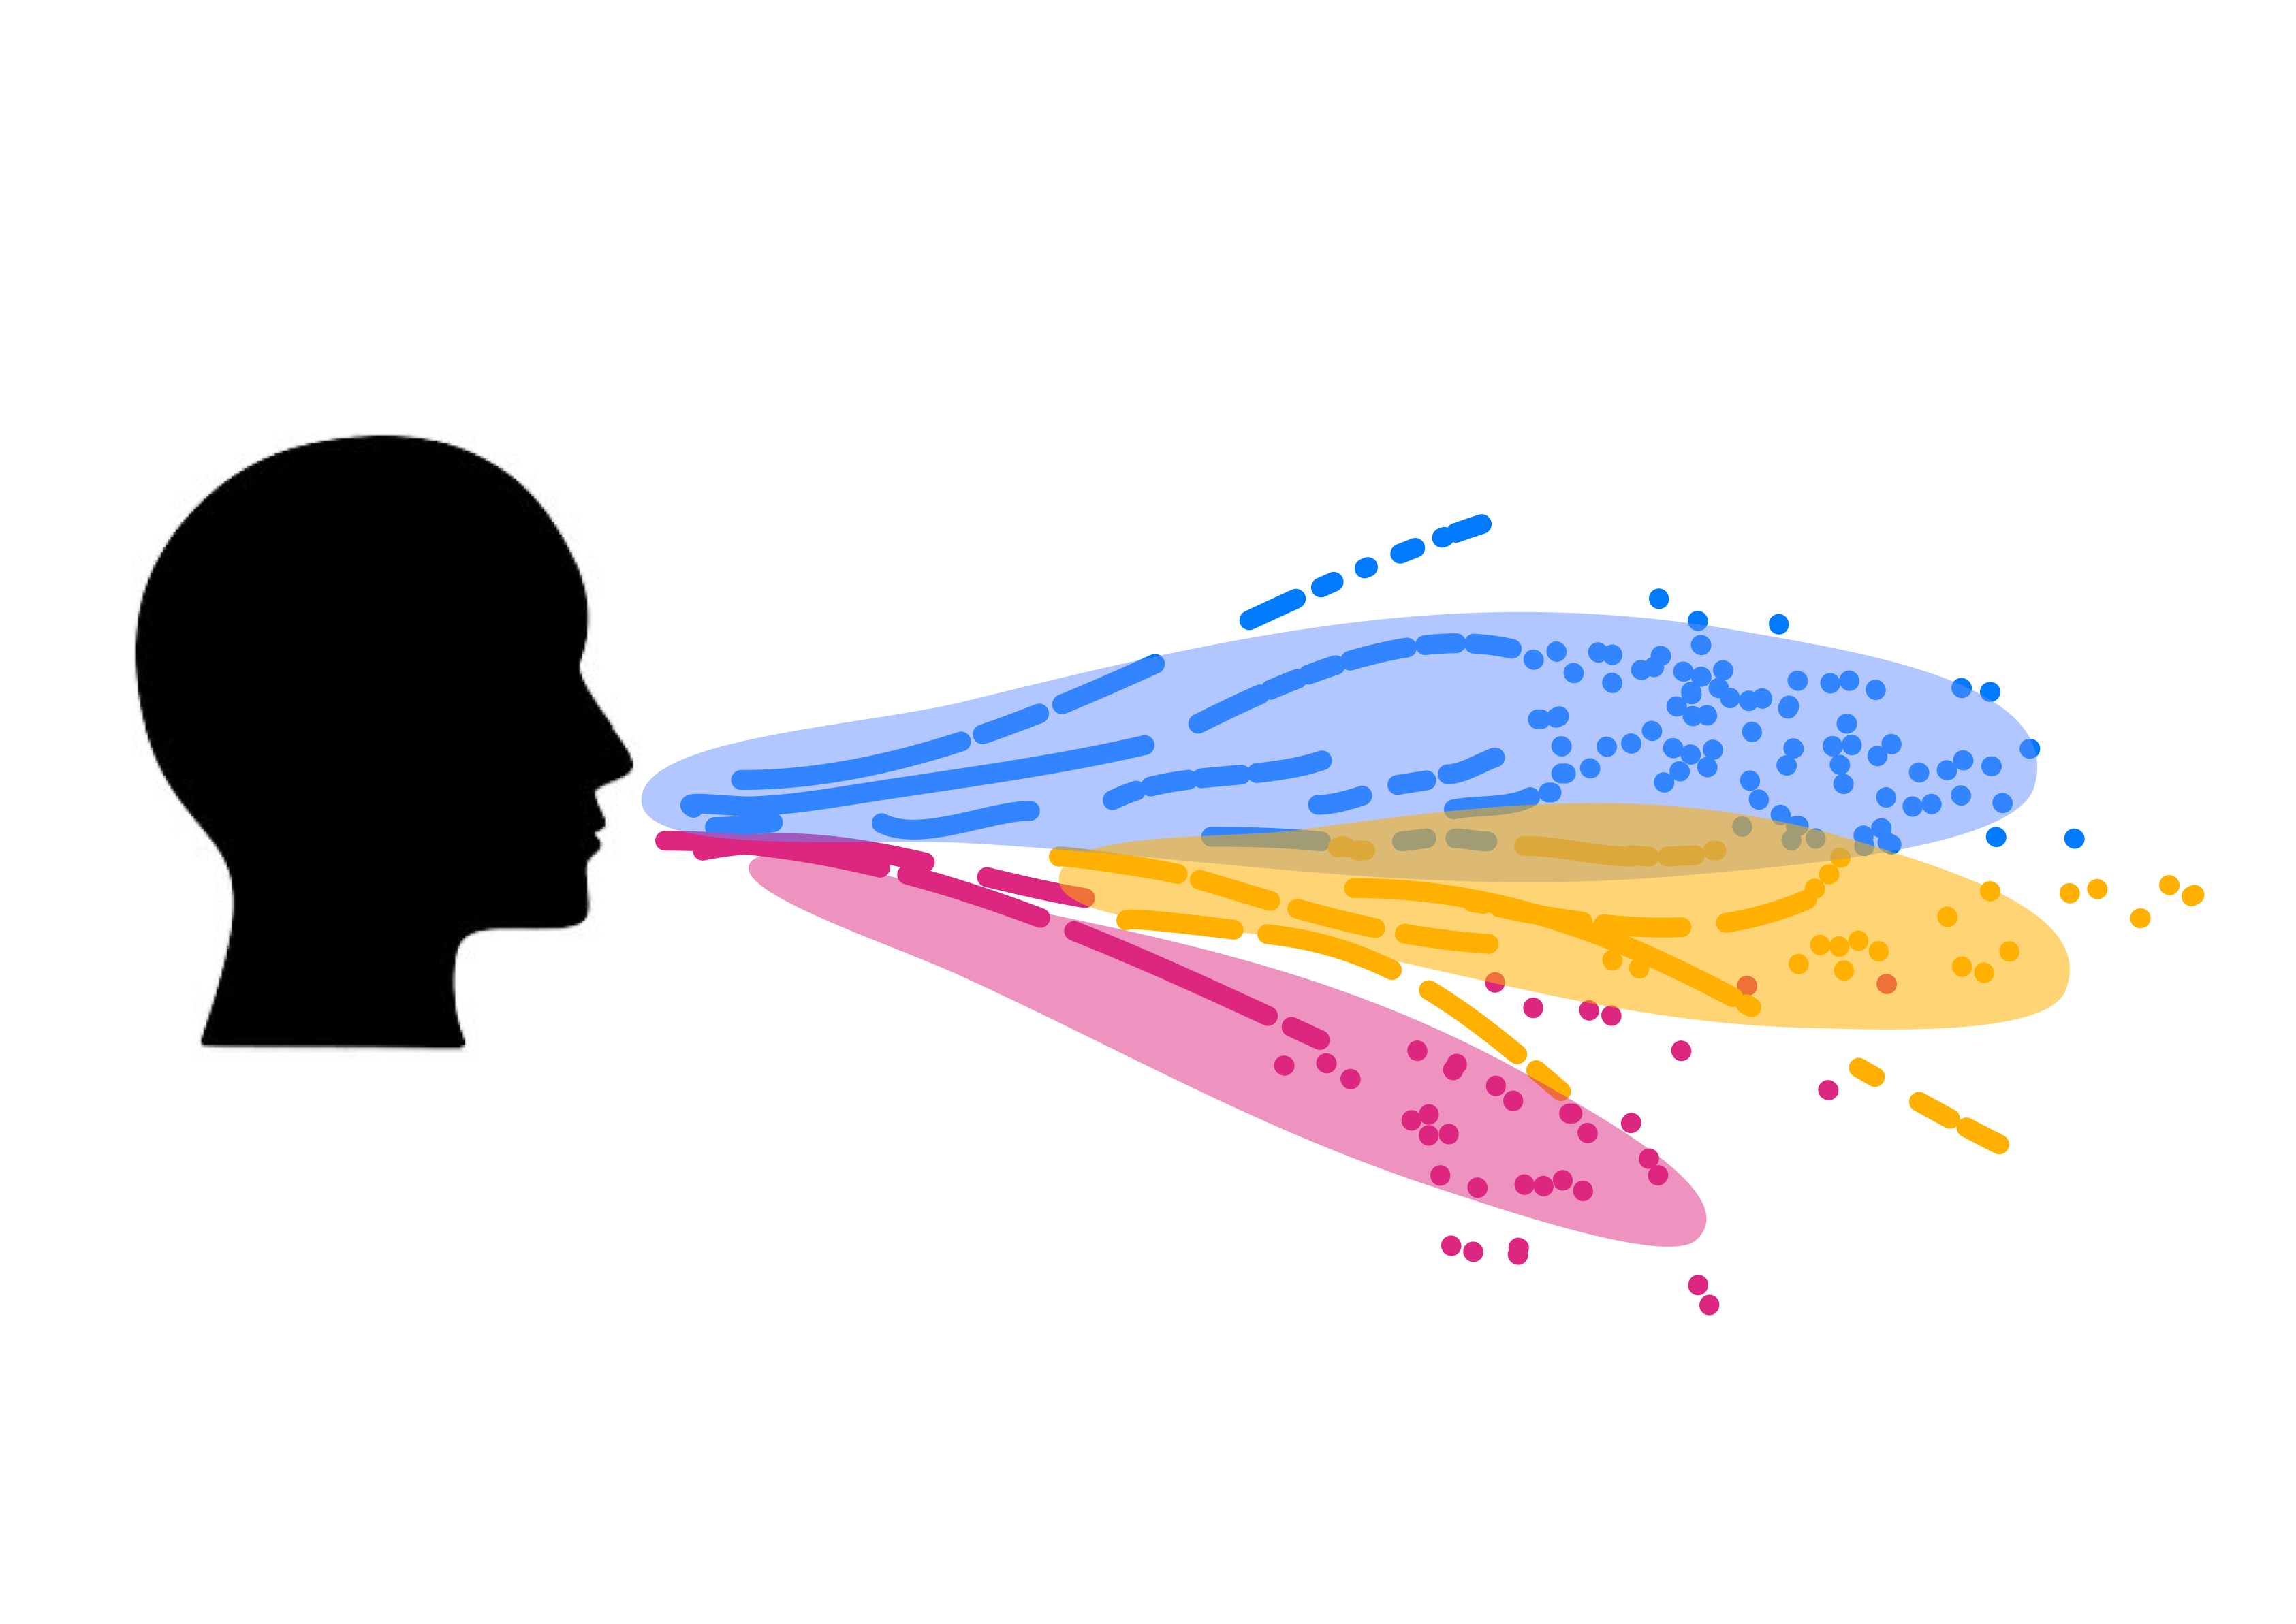
\includegraphics[clip,trim={0 2cm 0 2cm},width=0.25\textwidth]{Droplets/dropmat5.jpeg} \\
    \hline
    References & \cite{zhang2019distribution,feng2020study} & References & \cite{vuorinen2020modelling,diwan2020understanding,pendar2020numerical,lu2020reducing,rosti2020fluid,dbouk2020coughing,ren2021numerical,zhou2021experimental,sen2021transmission,mirzaie2021covid,chong2021extended,aliyu2021dispersion,yan2021transmission, lordly2022understanding,wang2022evaluation} \\
    \hline
    Low air temperature \& High humidity & 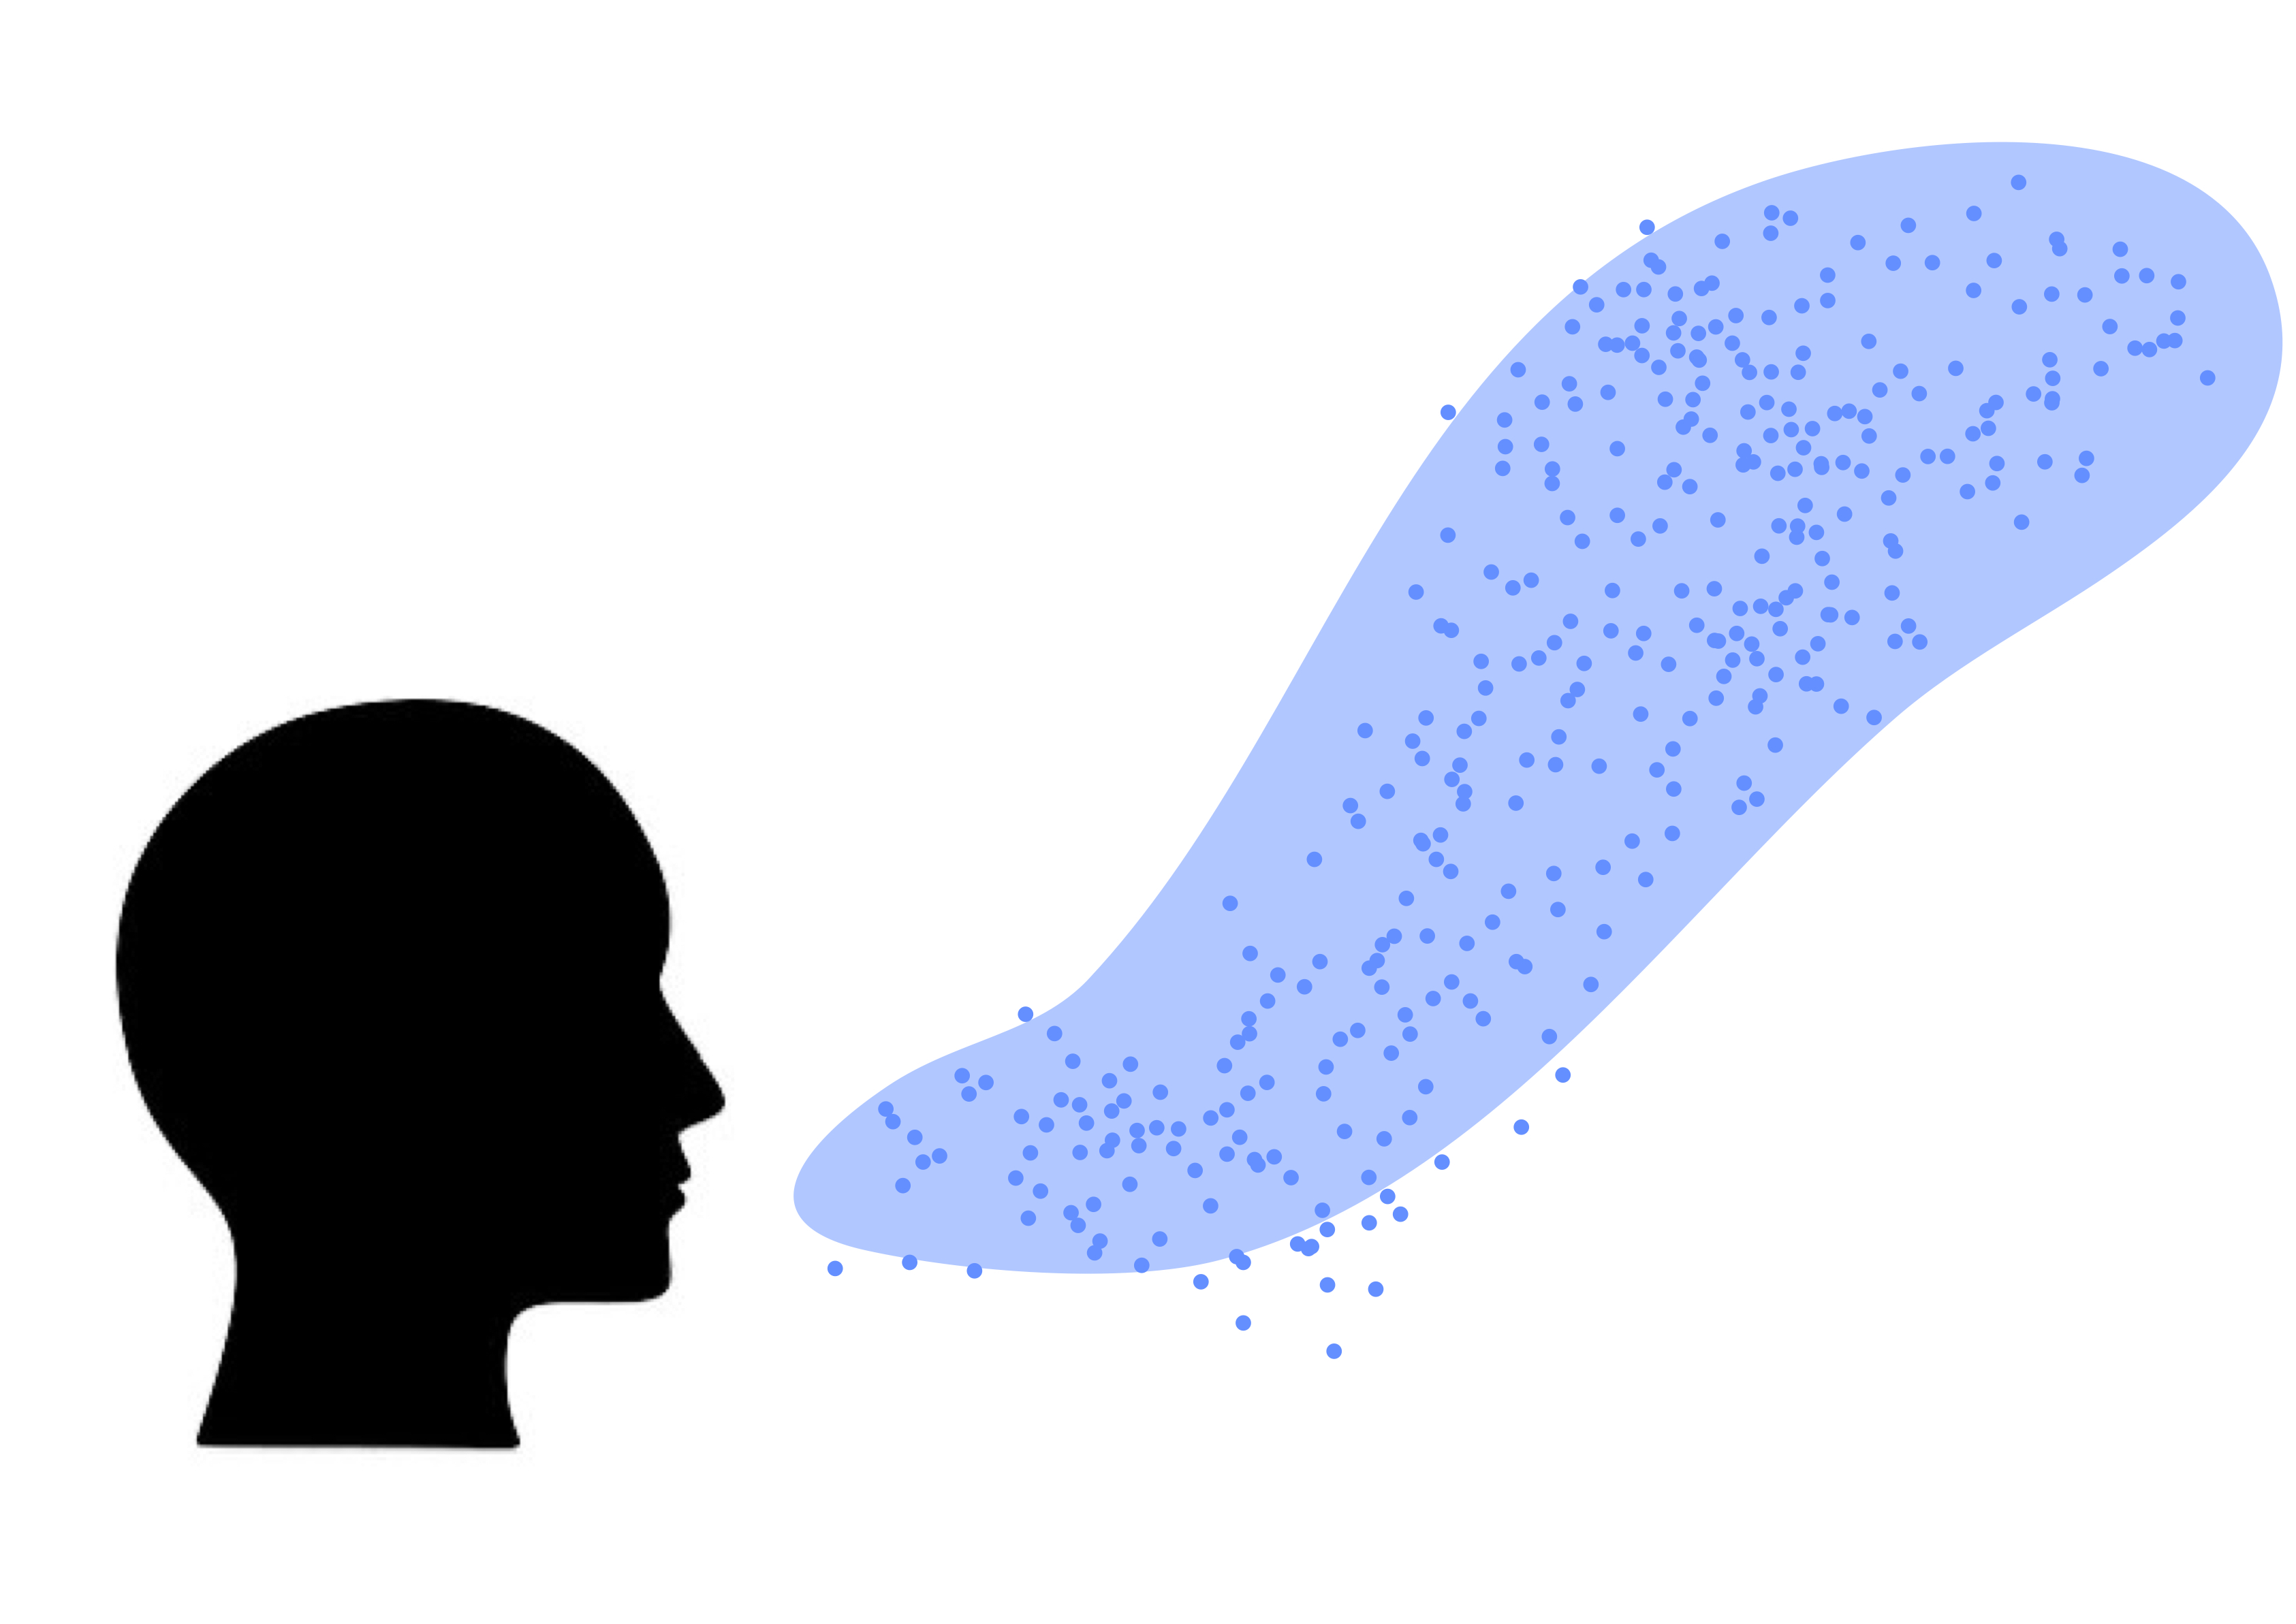
\includegraphics[clip,trim={0 2cm 0 2cm},width=0.25\textwidth]{Droplets/dropmat2.jpeg}& Sneezing & 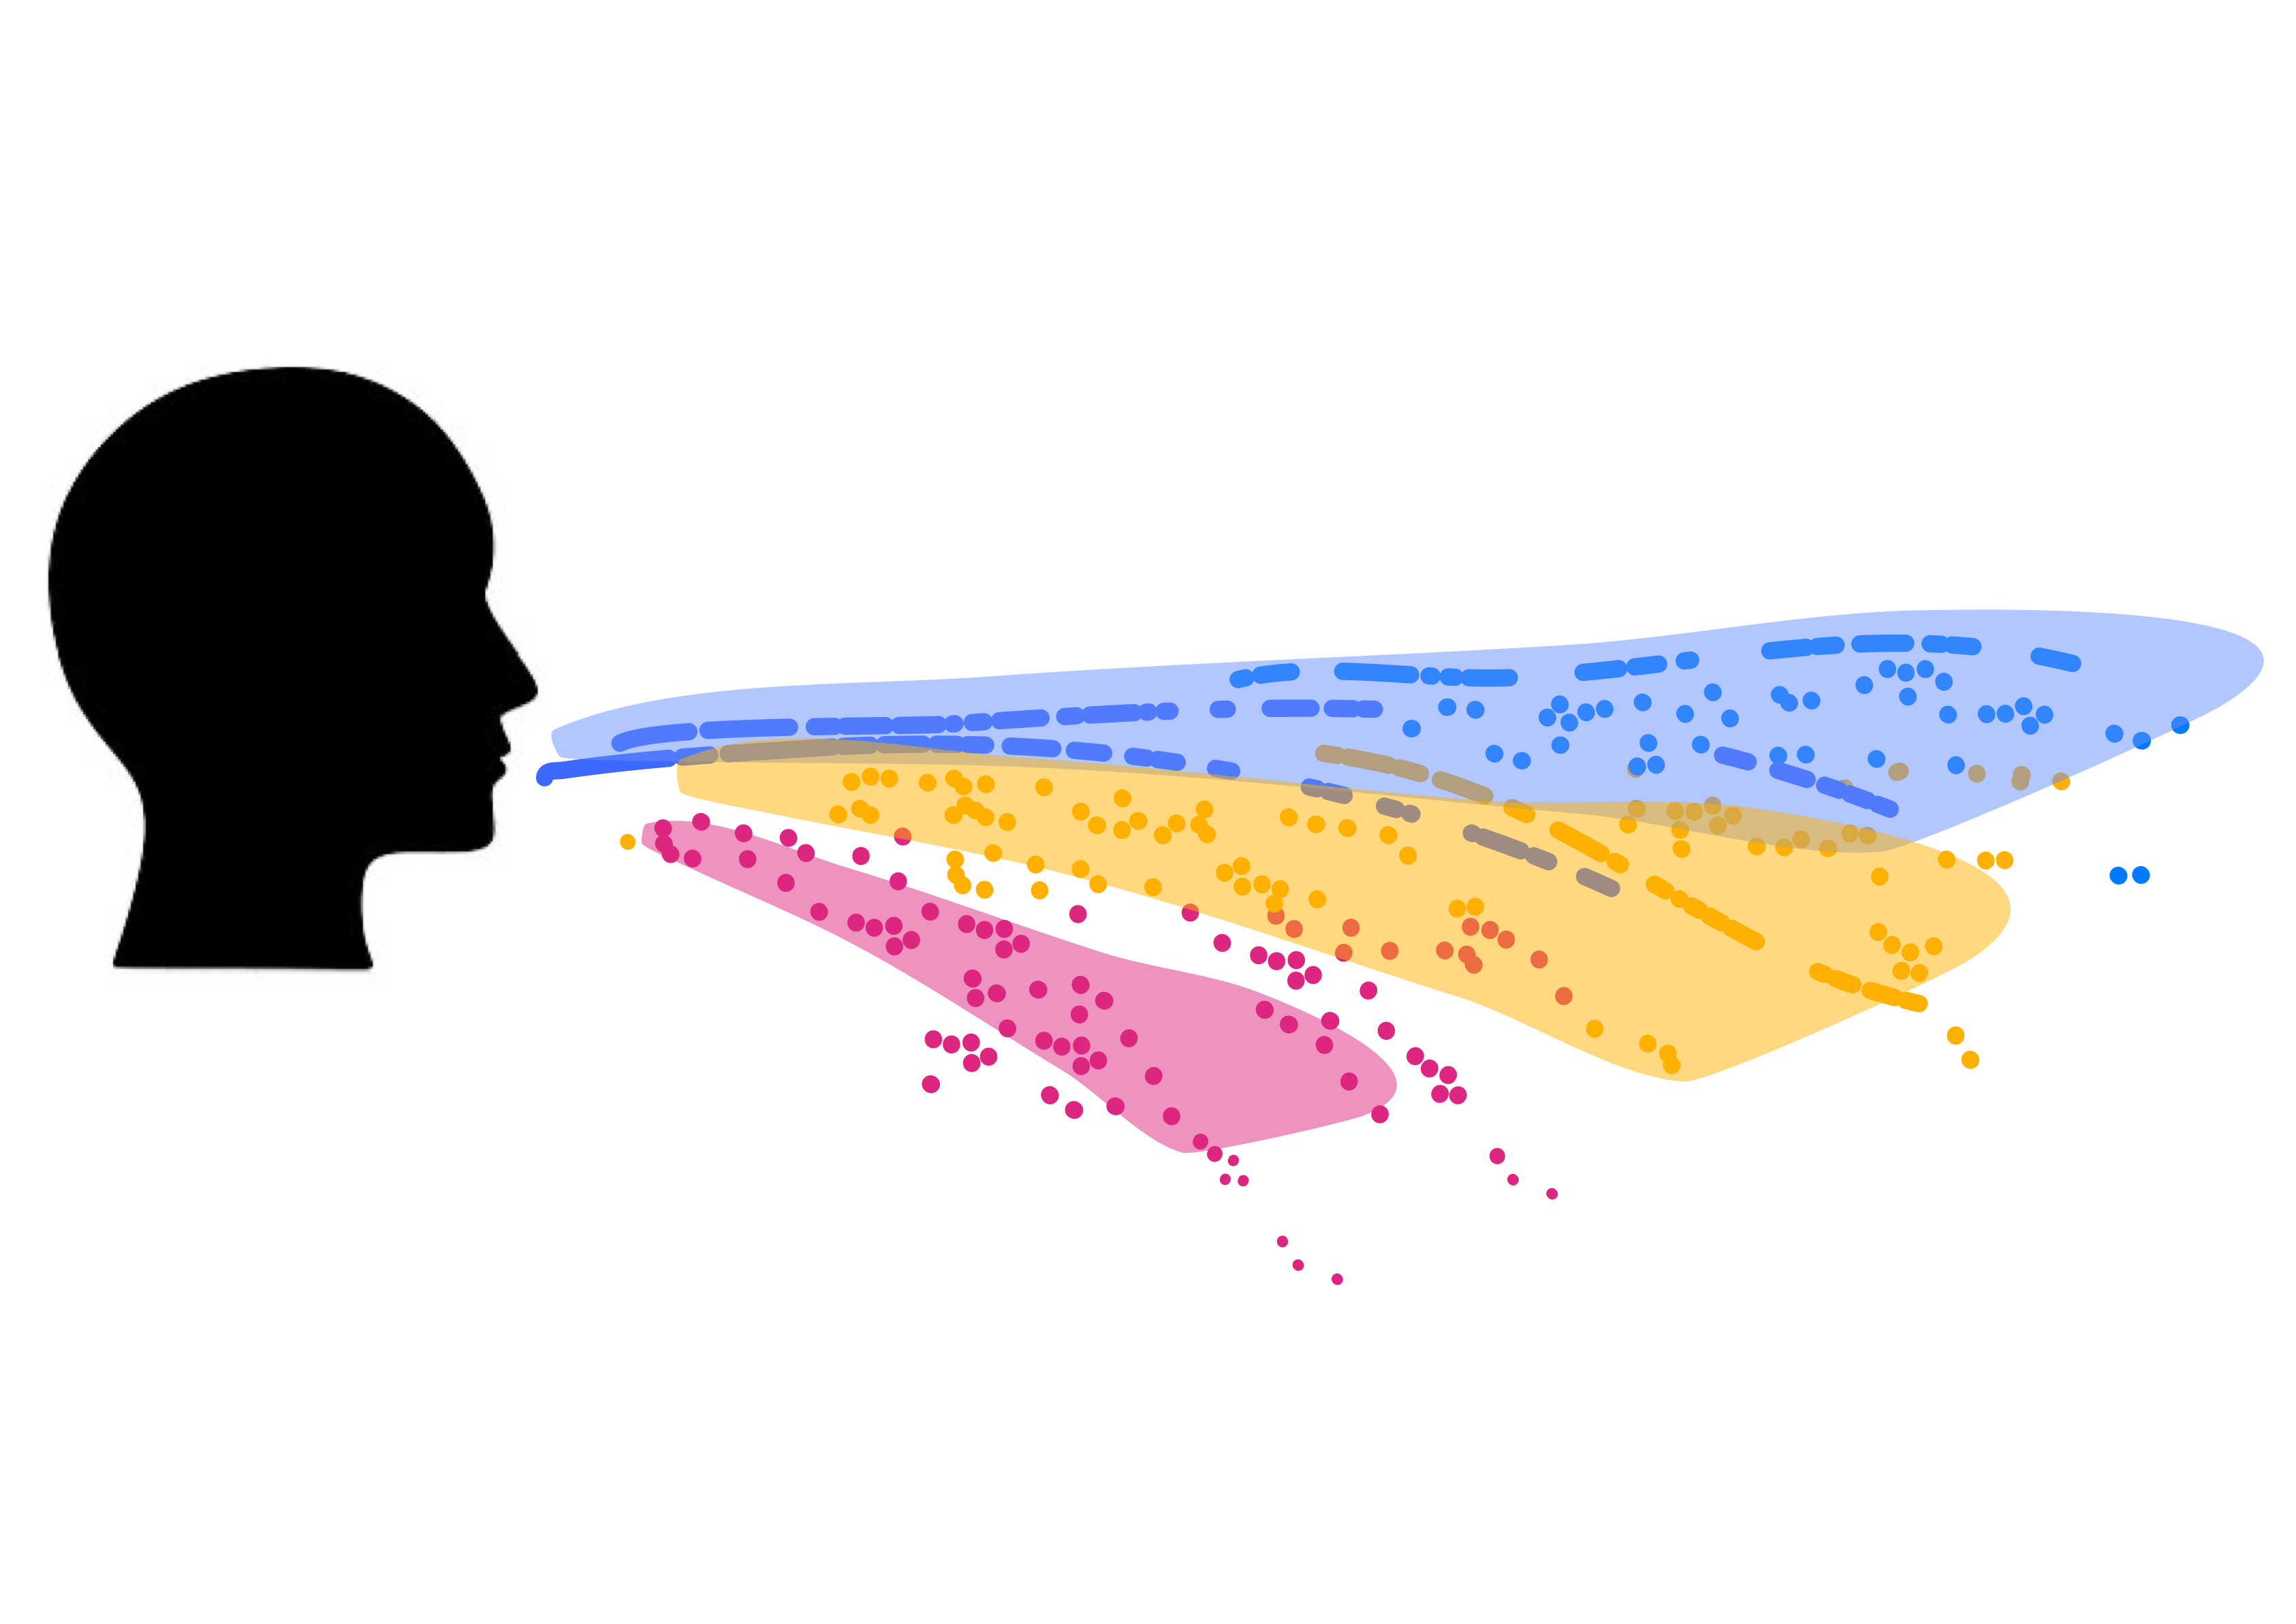
\includegraphics[clip,trim={0 2cm 0 2cm},width=0.25\textwidth]{Droplets/dropmat6.jpeg} \\
    \hline
    \textbf{References} & \cite{zhang2019distribution,chong2021extended} & \textbf{References} & \cite{pendar2020numerical,diwan2020understanding,fontes2020study,aliyu2021dispersion} \\
    \hline
    High air temperature \& Low humidity & 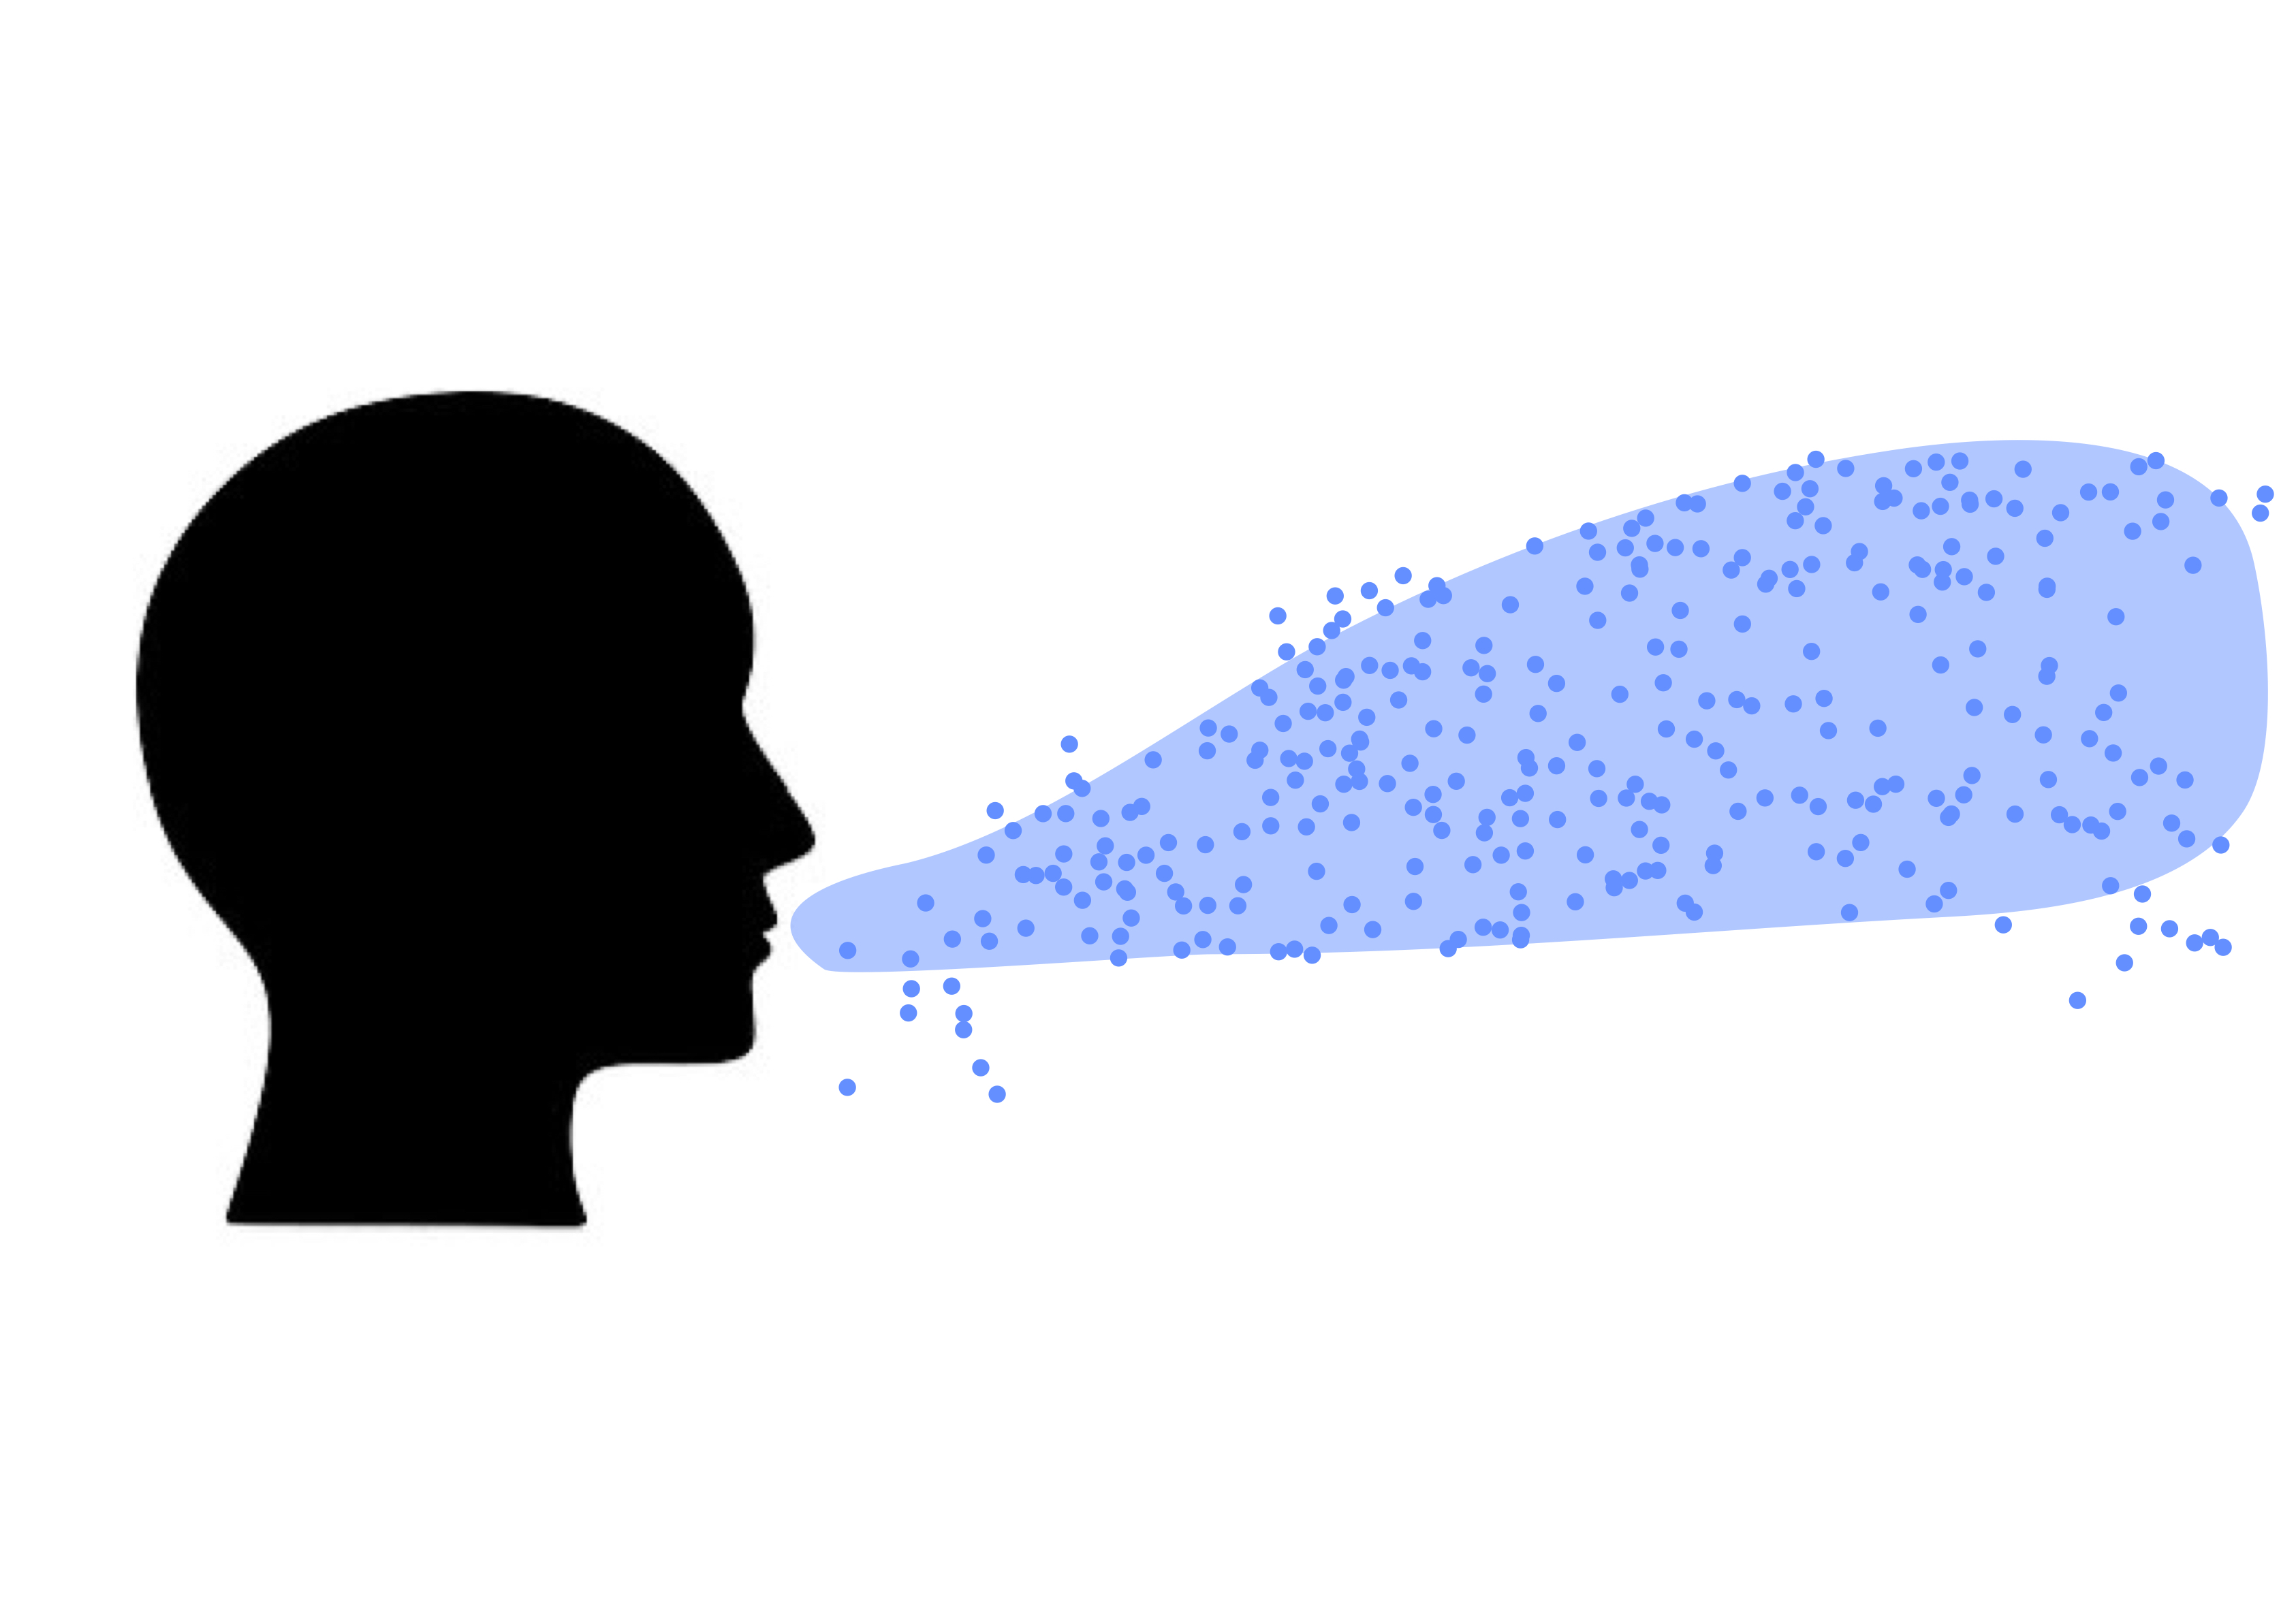
\includegraphics[clip,trim={0 2cm 0 2cm},width=0.25\textwidth]{Droplets/dropmat3.jpeg}& Breathing & 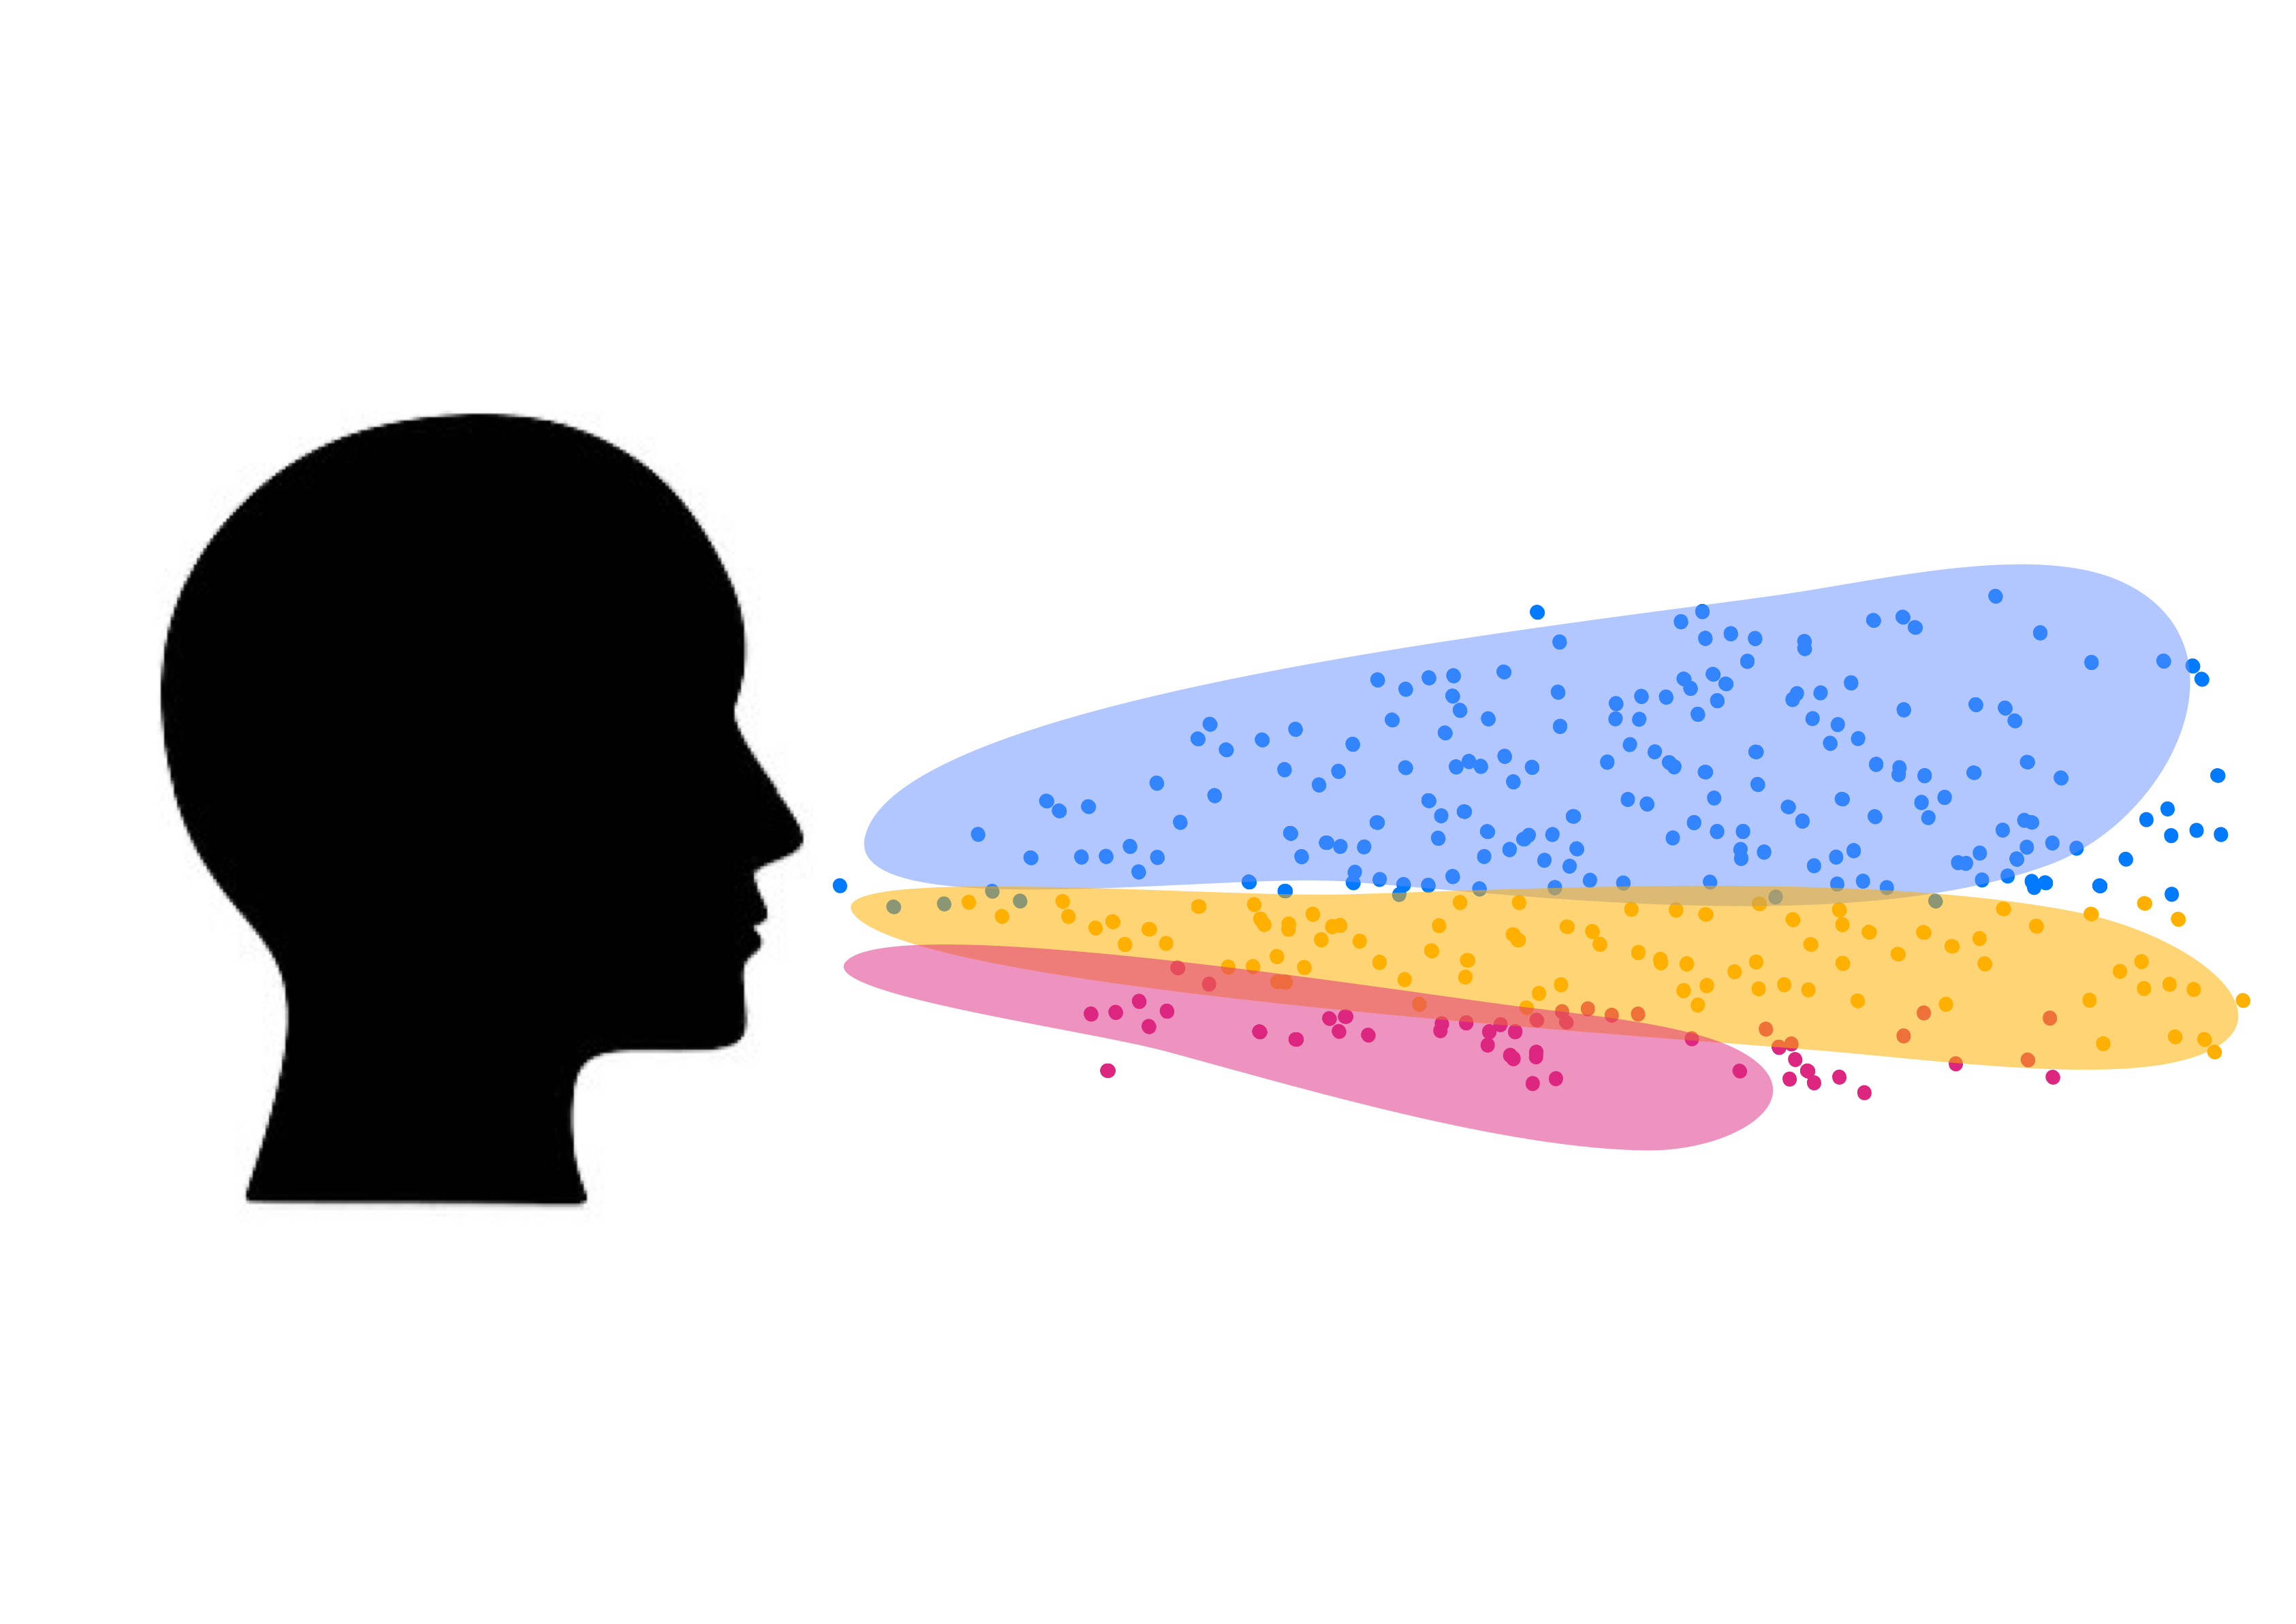
\includegraphics[clip,trim={0 2cm 0 2cm},width=0.25\textwidth]{Droplets/dropmat7.jpeg} \\
    \hline
    \textbf{References} & \cite{zhang2019distribution,feng2020study,sen2021transmission} & \textbf{References} & \cite{he2011cfd,villafruela2019assessment,duill2021impact,shao2021risk,luo2022role,wang2022evaluation,wei2023effects} \\
    \hline
   High air temperature \& High humidity & 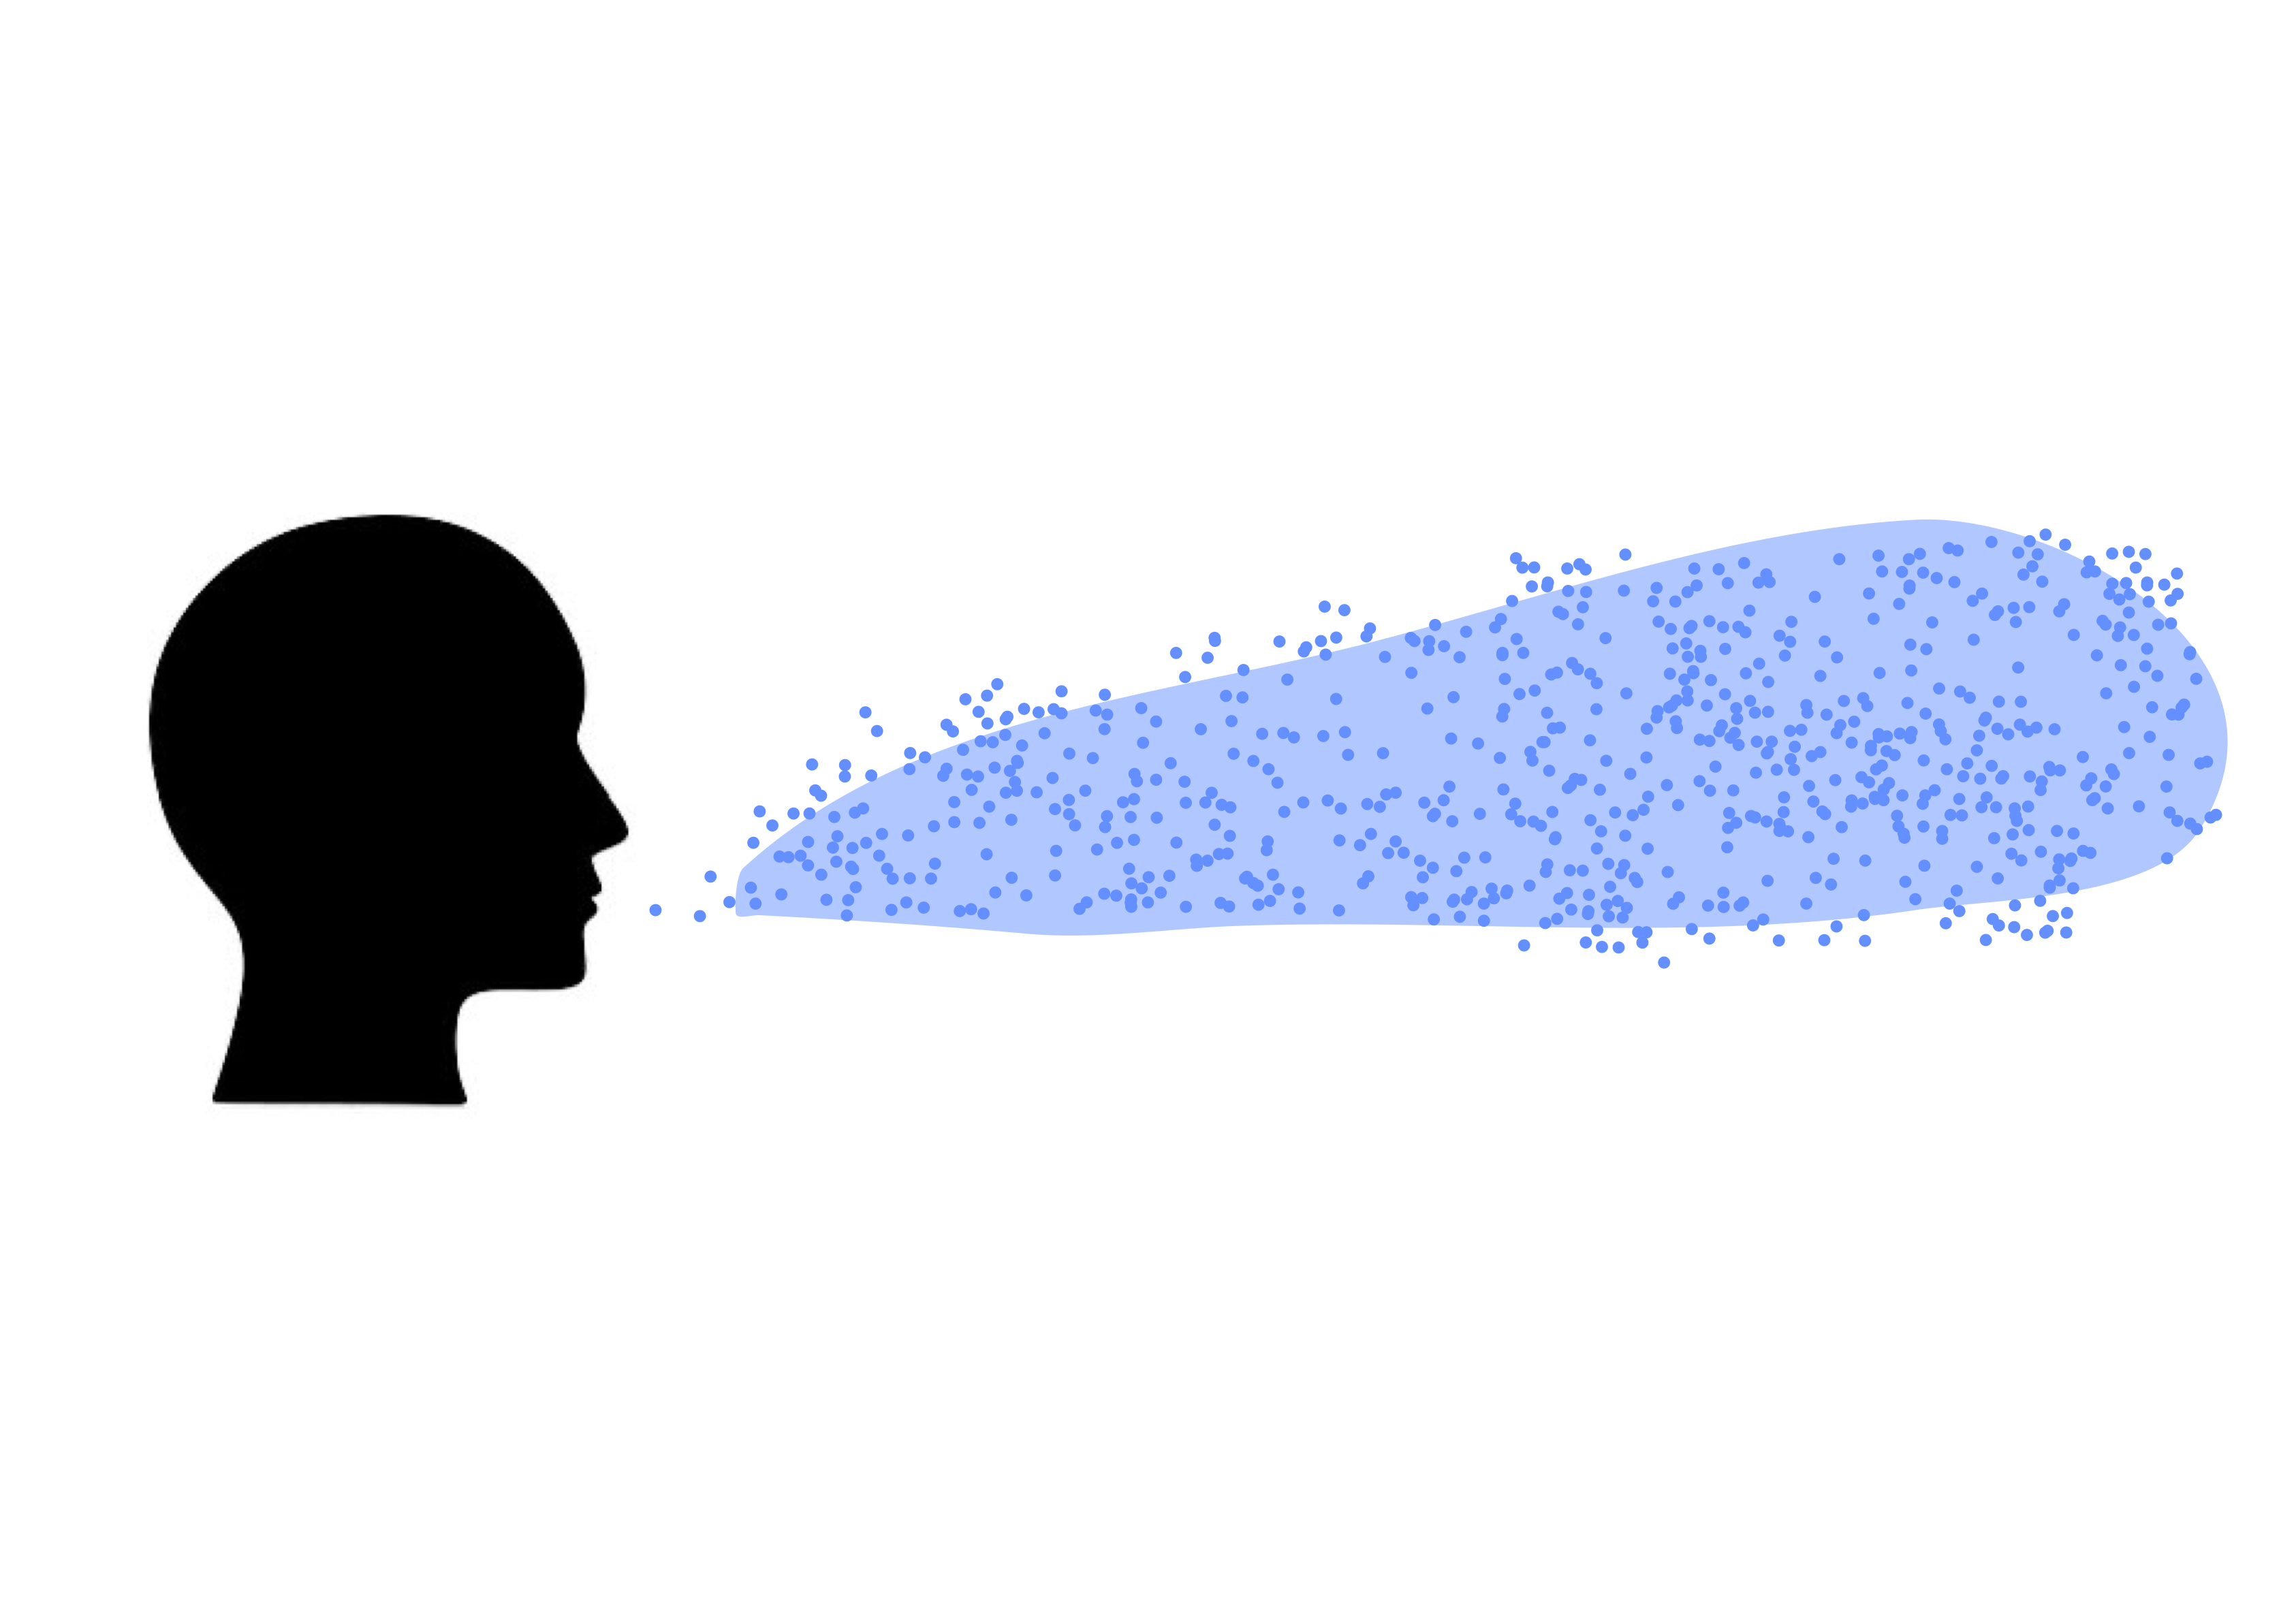
\includegraphics[clip,trim={0 2cm 0 2cm},width=0.25\textwidth]{Droplets/dropmat4.jpeg}& Speaking & 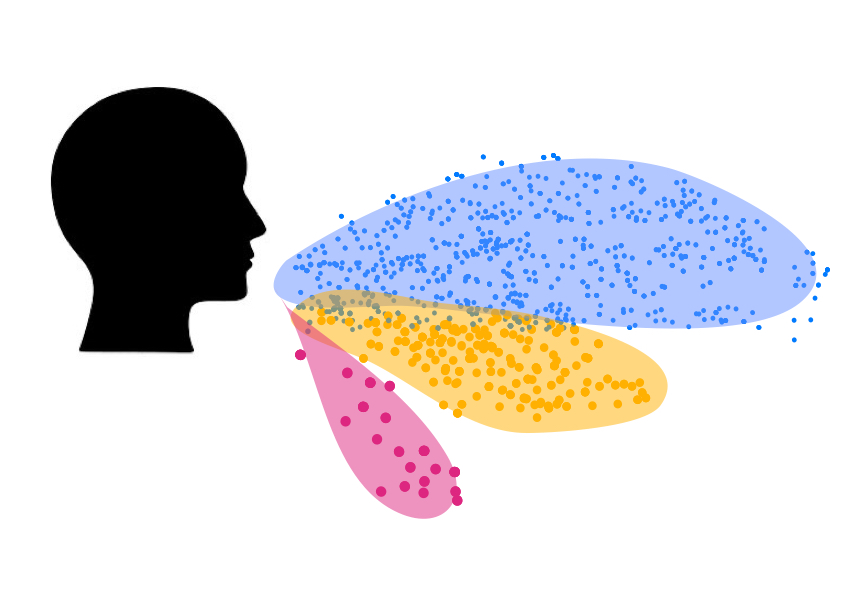
\includegraphics[clip,trim={0 2cm 0 2cm},width=0.25\textwidth]{Droplets/dropmat8.jpeg} \\
    \hline
    \textbf{References} & \cite{zhang2019distribution,chong2021extended} & \textbf{References} & \cite{vuorinen2020modelling,zhou2021experimental,wang2022evaluation,wei2023effects} \\
    \hline
    \end{tabular}
    \caption{Schematics of droplet plumes in different air conditions and respiratory activity.}
    \label{tab:mat2}
    \vspace{0.3cm}
    \normalsize
    NOTE: The different-sized droplets expelled during respiratory activities are shown as:\\ \legendsquare{fill=resp} Small droplets \legendsquare{fill=vent} Medium-sized droplets \legendsquare{fill=therm} Large droplets 
\end{table}

\subsection{Experimental and Numerical approaches}

Epidemiological studies were very successful in identifying the high spreading potential of SARS-CoV-2 \cite{rothan2020epidemiology} and previously provided strong evidence for airborne transmission of infectious diseases like Tuberculosis, chickenpox, SARS, measles, influenza, and smallpox. Since establishing a direct link between airflow patterns in an indoor environment and the transmission of infectious diseases, airflow studies simulating the transmission of pathogen-laden droplets have become more popular \cite{li2007role}. Ventilation design may be essential in reducing the droplet concentration near an occupant. 

The two approaches for achieving an optimal ventilation design are experimental and numerical. Laboratory measurements in climate chambers with tracer gases or artificially generated aerosols have been performed to obtain the particle distribution in the presence of ventilation and occupant flow \cite{zhou2021experimental}. On the other hand, computational methods try to simulate aerosol movement by modelling the turbulence in respiratory flow, ventilation flow, droplet physics, and thermal flow using Computational Fluid Dynamics (CFD) \cite{wang2022evaluation}. CFD is a more popular method for researchers because of its accessibility and repeatability compared to full-scale experiments. Experimental studies have often been used for validating the CFD results, e.g. \cite{yin2009experimental} is a popular benchmark for validating numerical results.

\subsubsection{Experiments in a controlled environment}

Mimicking airborne transmission in laboratory conditions involves accounting for numerous variables, making experiments challenging. Therefore, scaled-down \cite{poussou2010flow} or full-scale experiments with limited parameters \cite{luo2022role} are often more practical. Since scaled-down or limited full-scale experiments cannot be directly compared to extensive computational studies, they are frequently used to validate the numerical model \cite{li2020investigating,qin2023transmission,cortellessa2023effectiveness}. Full-scale experiments include an initial flow rate measurement at the ventilation supply to assign boundary conditions in the CFD simulations \cite{romano2015numerical}. Researchers have used different techniques to generate and measure the three major components of indoor airflow (i.e., respiratory jet, thermal plume, and ventilation flow), as shown in Table \ref{tab:exp}.

The studies listed in the first column of Table \ref{tab:exp} show experiments conducted to either validate or complement the results from the numerical simulations. These studies have utilised various strategies to mimic different sources of indoor airflow, as listed in the second column of Table \ref{tab:exp}. Aerosol generators, breathing manikins, or human test subjects have been used to mimic respiratory flow. The aerosol generators are either seeded with DEHS (Di-Ethyl-Hexyl-Sebacat) \cite{jain2023numerical} or bacteria \cite{liu2020full}, or virus \cite{oksanen2022combining}. For ventilation flow in a room, most of the studies make use of ventilation supply from real-life settings \cite{romano2015numerical,duill2021impact} or test chambers \cite{zhang2019distribution, berrouk2010experimental}. At times, air cleaners have been used with or without standard ventilation to generate ventilation flow in the room \cite{oksanen2022combining, jain2023numerical}. For mimicking thermal flows, thermal manikins \cite{li2021effects} or heaters \cite{ho2021modeling} are used. In some cases, human subjects are also involved in experiments for generating thermal flows \cite{li2005role, deng2021control}.

Depending on the different methods of generating flow and the purpose of the experiments, the flow parameters are measured using various techniques shown in the third column of Table \ref{tab:exp}. Some studies inject tracer gas like $SF_6$, or $N_2O$ at the origin of airflow \cite{qian2008dispersion, cheng2021experimental} or exhaled $CO_2$ gas as tracer \cite{deng2021control} and measure the spatial concentration of the gases using sensors. Aerosol generators using DEHS or other saline solutions that form fine droplets are usually measured using aerosol spectrometers \cite{duill2021impact}, optical particle counters \cite{berrouk2010experimental} or aerosol monitors \cite{zhou2021experimental}. While, nebulised bio-aerosol solutions are measured using Anderson Cascade Impactor (ACI), which samples bacteria or viruses from the air into petri dishes \cite{liu2020full,liu2020experimental}. For setting up the numerical model, flow meters are used to measure the flow rate at ventilation supplies \cite{li2005role,liu2023estimating} and for validating it, anemometers are used to measure the velocity and temperature of the airflow inside the room \cite{li2023numerical,arpino2023cfd}. A few experiments also use Particle Image Velocimetry (PIV) \cite{faleiros2022tu} or Planar Laser-Induced Fluorescence (PLIF) \cite{poussou2010flow} to quantify the velocity and concentration fields, respectively.

\begin{center}
\captionsetup{font=normalsize}
\footnotesize
\LTcapwidth=\textwidth
\begin{longtable}{|m{3.55cm}|m{3.5cm}|m{3.5cm}|m{3.5cm}|}
\caption{Brief breakdown of experimental techniques in previous literature}
\label{tab:exp}\\
    \hline
    \centering\textbf{Studies} & \centering\textbf{Flow generation method} & \centering \textbf{Measurement method} & \centering\textbf{Type of flow}\\
    \hline
    \citet{berrouk2010experimental}& Aerosol spray gun, ventilation and thermal manikin & Anemometer and Particle counter & Respiratory, ventilation and thermal\\
    \hline
    \citet{li2005role} & Ward patients and ventilation & Flow meters & Respiratory, ventilation, and thermal\\
    \hline
    \citet{saarinen2015large} & Manikin dynamics & Tracer gas & Room air escape \\
    \hline
    \citet{jiang2009investigating}& External wind & Tracer gas & Ventilation\\
    \hline
    \citet{faleiros2022tu}& A male subject & PIV & Respiratory and thermal\\
    \hline
    \citet{romano2015numerical}& Ventilation and Nebuliser & Particle counters and Anemometers & Respiratory and ventilation\\
    \hline
    \citet{quintero2022reducing}& Atomiser & Particle counters & Ventilation \\
    \hline
    \citet{hang2015potential}& Thermal manikin and ventilation & Tracer gas & Respiratory, ventilation, and thermal \\
    \hline
    \citet{jain2023numerical}& Air cleaner & Aerosol generator and spectrometers & Ventilation \\
    \hline
    \citet{li2023numerical}& Ventilation and thermal manikin & Anemometers  & Ventilation and thermal \\
    \hline
    \citet{ho2021modeling}& On-board heater & Anemometers & Thermal\\
    \hline
    \citet{deng2021control}& Two test subjects and air conditioning system & Exhaled $CO_2$ as tracer gas & Respiratory, ventilation and thermal\\
    \hline
    \citet{oksanen2022combining}& Ventilation, air cleaner and Nebuliser & ACI sampler and aerosol spectrometer & Ventilation and thermal\\
    \hline
    \citet{arpino2023cfd}& Ceiling diffusers & Anemometers & Ventilation \\
    \hline
    \citet{giri2022colliding}& Smoke generator & Flow visualisation & Respiratory\\
    \hline
    \citet{liu2020experimental}& Ventilation and Bio-aerosol release & ACI sampler and plate counting & Ventilation and thermal \\
    \hline
    \citet{qian2008dispersion}& Breathing manikins & Tracer gas & Respiratory\\
    \hline
    \citet{lu2020reducing}& Ventilation & Tracer gas & Ventilation\\
    \hline
    \citet{poussou2010flow}& Ventilation and moving body & PIV and PLIF & Ventilation \\
    \hline
    \citet{liu2020full}& Bio-aerosol generator and ventilation & Anemometers and ACI & Respiratory and Ventilation \\
    \hline
    \citet{cheng2021experimental}& Breathing thermal manikin & Tracer gas & Ventilation, respiratory and thermal\\
    \hline
    \citet{liu2023estimating}& Bio-aerosol generator and ventilation & ACI and flowmeter & Respiratory and ventilation \\
    \hline
    \citet{li2021effects}& Breathing thermal manikin & Tracer gas & Respiratory, ventilation, and thermal\\
    \hline
    \citet{duill2021impact}& Test subjects and Air cleaner &  Aerosol spectrometer & Respiratory and Ventilation\\
    \hline
    \citet{zhou2021experimental}& Thermal manikin, aerosol generator, and ventilation  & Aerosol monitor & Respiratory, ventilation, and thermal \\
    \hline
    \citet{zhang2019distribution}& Ventilation, Thermal manikin, and Aerosol generator & Aerosol monitor & Respiratory, ventilation, and thermal\\
    \hline
\end{longtable}
\end{center}

\subsubsection{Numerical simulations}

While experimental techniques use anemometers, sensors, flowmeters, and visualisation methods, Computational Fluid Dynamics (CFD) is a numerical approach that uses computer processors to solve fluid flow problems. CFD uses codes that discretise the Navier Stokes equation into algebraic equations and solve them iteratively \cite{ferziger2002computational}. Commercially available codes like Ansys \cite{ANSYS}, STAR-CCM+ \cite{starccm}, ABAQUS \cite{abaqus} and open-source codes like OpenFOAM \cite{openfoam}, SU2 \cite{su2}, xcompact3D \cite{xcompact3d}, PALM \cite{palm}. There are three approaches to numerical simulations (from low to high fidelity in turbulence representation): Reynold Averaged Navier Stokes (RANS), Large Eddy Simulations (LES), and Direct Numerical Simulations (DNS).

RANS averages the NS equations over time, using Reynolds decomposition,
giving a Reynolds stress tensor term \cite{wilcox2006turbulence}. This term represents the effect of turbulence, which is assumed to be statistically steady and is modelled using k-$\epsilon$ or k-$\omega$ models \cite{pope2000turbulent}. In contrast to RANS, LES resolves the larger, energy-containing eddies while modelling the smaller, dissipative eddies \cite{sagaut2006large}. It is useful for complex flow applications where it is important to resolve the large turbulent structures \cite{smagorinsky1963general}. DNS directly computes the entire range of turbulent scales rather than modelling it like in RANS, making it computationally expensive \cite{moin2011dns}. 

Table \ref{tab:num} categorises the reviewed studies according to their numerical approach; a decreasing number of studies can be observed moving from RANS to DNS. This decrease is because of the high computational resources required for LES and DNS and the ease of running commercially available RANS codes. Among the RANS studies, the most used turbulence models are k-$\epsilon$ \cite{ren2021numerical,ou2022insufficient} and k-$\omega$ SST \cite{dbouk2020coughing,yan2021transmission}. ANSYS Fluent is often used to perform indoor RANS simulations with additional modelling for droplet physics \cite{li2020investigating,wei2023effects}. In the following column, the studies have resolved the most energetic turbulent eddies and modelled the subgrid scales using the Wall Adapting Local Eddy (WALE) viscosity model \cite{feng2020study,zhang2019distribution}, Smagorinsky Lilly model \cite{wu2023numerical,li2022airborne}, and one equation eddy viscosity model \cite{pendar2020numerical}. The codes used to perform LES are a mix of commercially available tools like Ansys \cite{saarinen2015large,feng2020study} and open-source tools like OpenFOAM and PALM \cite{vuorinen2020modelling}. In the last column, studies have resolved all turbulent scales with the help of bespoke codes like AFiD \cite{chong2021extended}, xcompact3D \cite{giri2022colliding}, Fujin \cite{rosti2020fluid}, Megha-5 \cite{singhal2022virus} etc.

\begin{center}
\captionsetup{font=normalsize}
\footnotesize
\LTcapwidth=\textwidth
\begin{longtable}{|m{3cm}|m{4.3cm}|m{4.4cm}|m{3.2cm}|}
    \caption{Numerical studies classified based on varying levels of resolving turbulent scales}
    \label{tab:num}\\
    \hline
    \centering \textbf{Simulation type} & \centering \textbf{RANS} & \centering \textbf{LES} & \center \textbf{DNS} \\
    \hline
    \centering \textbf{Studies} & \citet{ren2021numerical} & \citet{feng2020study} & \citet{giri2022colliding} \\
    
     & \citet{li2020investigating} & \citet{khosronejad2020fluid} & \citet{chong2021extended} \\
    
     & \citet{dbouk2020respiratory} & \citet{zhang2019distribution} & \citet{diwan2020understanding} \\
    
     & \citet{liu2020experimental} & \citet{berrouk2010experimental} & \citet{singhal2022virus} \\
    
     & \citet{dbouk2020coughing} & \citet{pendar2020numerical} & \citet{rosti2020fluid} \\
    
     & \citet{aliyu2021dispersion} & \citet{abkarian2020speech} &  \\
    
     & \citet{zhou2021experimental} & \citet{saarinen2015large} &  \\
    
     & \citet{mirzaie2021covid} & \citet{li2023transient} &  \\
    
     & \citet{qian2008dispersion} & \citet{liu2021simulation} &  \\
    
     & \citet{li2005role} & \citet{quintero2022reducing} &  \\
    
     & \citet{villafruela2019assessment} & \citet{buchan2020predicting} &  \\
    
     & \citet{he2011cfd} & \citet{wu2023numerical} &  \\
    
     & \citet{jiang2009investigating} & \citet{fontes2020study}* &  \\
    
     & \citet{yan2021transmission} & \citet{salinas2022improved} &  \\
    
     & \citet{ren2021numerical} & \citet{krishnaprasad2023fluid} &  \\
    
     & \citet{faleiros2022tu} & \citet{vuorinen2020modelling} &  \\
    
     & \citet{romano2015numerical} & \citet{liu2023estimating} &  \\
    
     & \citet{lu2022ventilation} & \citet{oksanen2022combining} &  \\
    
     & \citet{lordly2022understanding} & \citet{li2022airborne} &  \\
    
     & \citet{guo2022visualization} & \citet{auvinen2022high} &  \\
    
     & \citet{qin2023transmission} &  &  \\
    
     & \citet{hang2014influence} &  &  \\
    
     & \citet{lu2020reducing} &  &  \\
    
     & \citet{pan2023predicting} &  &  \\
    
     & \citet{hang2015potential} &  &  \\
    
     & \citet{wu2023numerical} &  &  \\
    
     & \citet{liu2022numerical} &  &  \\
    
     & \citet{li2023numerical} &  &  \\
    
     & \citet{poussou2010flow} &  &  \\
    
     & \citet{luo2022role} &  &  \\
    
     & \citet{shao2021risk} &  &  \\
    
     & \citet{liu2019modeling} &  &  \\
    
     & \citet{ho2021modeling} &  &  \\
    
     & \citet{ou2022insufficient} &  &  \\
    
     & \citet{liu2020full} &  &  \\
    
     & \citet{cheng2021experimental} &  &  \\
    
     & \citet{wang2022evaluation} &  &  \\
    
     & \citet{liu2023estimating} &  &  \\
    
     & \citet{wei2023effects} &  &  \\
    
     & \citet{li2021effects} &  &  \\
    
     & \citet{cortellessa2023effectiveness} &  &  \\
    
     & \citet{srivastava2021effective} &  &  \\

     & \citet{deng2021control} &  &  \\
   
     & \citet{xu2023cfd} &  &  \\
    
     & \citet{motamedi2022cfd} &  &  \\
    
     & \citet{arpino2023cfd} &  &  \\
    
     & \citet{pan2022boundary} &  &  \\
    
     & \citet{yang2021airborne} &  &  \\
     & \citet{sen2021transmission} &  &  \\
     & \citet{feng2020influence} &  &  \\
     & \citet{fontes2020study}* &  &  \\
    \hline
\end{longtable}
* Detached Eddy Simulation with both RANS and LES approaches used
\end{center}

\section{Discussion}


\subsection{Ventilation regime and setting}
From Table \ref{tab:mat}, it is evident that Ventilation regime 1 is the most widely used ventilation regime across all occupant configurations and almost all indoor settings. This is supported by the fact that mixing ventilation can dilute the pathogen or pollutant concentration in the room \cite{srivastava2021effective}. Ventilation regimes 2 and 3 are less common in comparison because the indoor airflow is directional, upward and lateral, respectively, making them less versatile in most scenarios but more effective in some. In some healthcare settings, a ventilation regime where the air is supplied vertically downwards is also implemented to deposit the suspended infectious aerosols on surfaces immediately \cite{lu2022ventilation,lu2020reducing, liu2020full}. Among the papers reviewed, Occupant Configuration 1, i.e., face-to-face occupant configuration, has received the least attention compared to the other occupant configurations. These occupant configurations are mostly found in restaurants, offices, and hospitals.

It was found that approximately 40\% of the reviewed studies do not replicate a specific indoor setting, and the rest barely consider social settings, especially restaurants. This is clearly illustrated in Figure \ref{fig:pie} for restaurant settings, making up a measly 3\% of the studies. Most studies focus on settings immediately affected by an outbreak, like healthcare settings (26\%), or have vulnerable occupants, like classroom settings (14\%). Office and transport settings constitute a total of 17\% of the reviewed studies. The fact that these settings have received priority over restaurant settings can be attributed to the fact that almost 80\% of the studies were conducted after the onset of the COVID-19 pandemic. However, there are no more restrictions on social gatherings in public places like restaurants, cafes, and bars, making these settings susceptible to massive spreading events in the case of a future outbreak.

\begin{figure}[ht]
\captionsetup{font=normalsize}
    \centering
    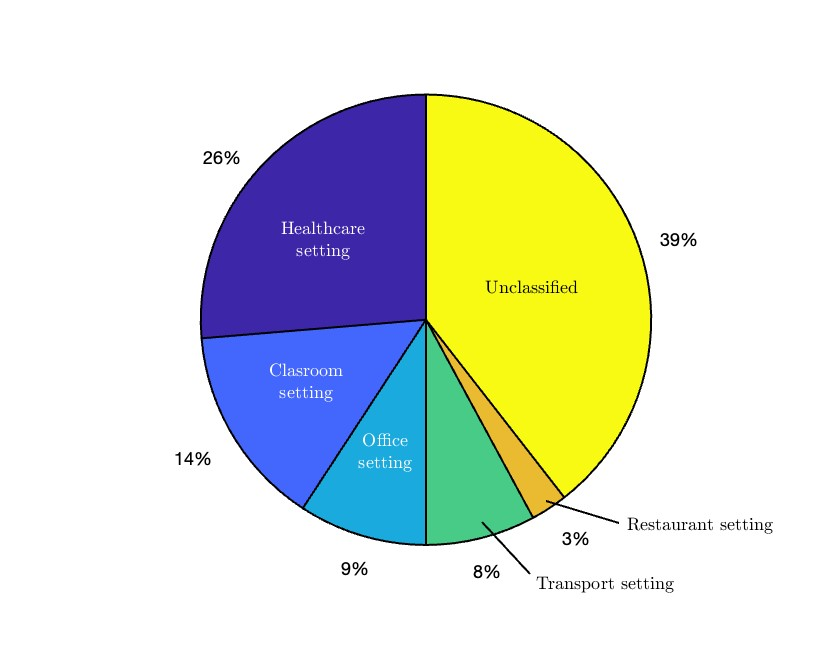
\includegraphics[width=0.75\textwidth]{figures/pie.jpg}
    \caption{Pie chart describing the lack of attention to restaurant settings}
    \label{fig:pie}
\end{figure}

\subsection{Indoor air conditions and respiratory activities}

In Table \ref{tab:mat2}, The first couple of columns compare the four different combinations of air conditions, while the next two compare the different respiratory activities. Among the reviewed studies, very few looked at air conditions as a combination of various air temperatures and RH. The respiratory flow behaves differently in different conditions that might alter the spatial concentration of the droplets in the room. Concerning the concentration of pathogen-laden droplets, the air conditions could affect the risk of exposure for a susceptible occupant inside a room. This makes the room's air conditions an essential factor to consider when minimising exposure risk for occupants.

On the other hand, numerous studies referring to one of the four respiratory activities in Table \ref{tab:mat2}, especially for coughing and breathing while sneezing and speaking, haven't received that much attention. As mentioned before, since most of the research papers reviewed in this study are from after the onset of the COVID-19 pandemic, more focus was put on coughing for short-range and breathing for long-range transmission. Now that people are more likely to interact in social gatherings, speech has become an essential respiratory activity that should be considered in both short-range and long-range airborne transmission in conjunction with ventilation. Speaking generates more droplets than other respiratory activities \cite{giri2022colliding}, significantly affecting a susceptible occupant's exposure risk. A combination of speaking and breathing is the most relevant in a social setting.

\subsection{Investigation approaches}

The airflow and droplet distribution in an indoor setting is usually mimicked using experimental or numerical approaches. In Table \ref{tab:exp}, all the experimental studies are broken down into the method of flow generation, method of measurement, and the flow type mimicked. Very few studies account for the three significant sources of airflow in their experiments \cite{zhou2021experimental,zhang2019distribution}. Anemometers are the common choice of apparatus for measuring airflow parameters like velocity and temperature, while particle concentrations are measured using tracer gas sensors and particle counters. Tracer gases are good at providing insight into airborne transmission through very fine droplets but fail to replicate the behaviour of two-phase respiratory flow. This shortcoming can be addressed using aerosol generators that nebulise pathogen-containing solutions, which are the most accurate way to mimic respiratory aerosol. Moreover, conventional tracer gases are visually undetectable; therefore, they do not provide any visual cues for how respiratory flow evolves. Few studies address this issue by using optical methods like smoke flow visualisation \cite{saarinen2015large,giri2022colliding}, soap bubbles visualisation \cite{bluyssen2021effect}, fluorescent tracking liquid with UV-lights \cite{ortiz2022testing}, and PIV/PLIF \cite{faleiros2022tu,poussou2010flow} to study the flow in the laboratory qualitatively. PIV and PLIF are also non-intrusive velocity and concentration measurement methods, making them ideal for studying aerosol droplets and the effect of ventilation and thermal flows on respiratory aerosol flow.

In Table \ref{tab:num}, the numerical studies are classified based on their approach towards resolving the turbulent structures in the simulated flow. The sheer difference in number is better illustrated in Figure \ref{fig:cfd}, which can be explained by the fact that RANS simulations are not computationally demanding and correlate with experimental results well enough in non-separating flows \cite{wu2023numerical}. RANS involves modelling the turbulent kinetic energy and turbulent dissipation as $k-\epsilon$ and $k-\omega$ turbulence models, where $k$ is the turbulent kinetic energy, $\epsilon$ is the turbulent dissipation, and $\omega$ is the specific rate of turbulent dissipation. These are some of the most widely used models in research and industry. In this review, 38 of the 51 RANS studies have performed RANS simulations with the $k-\epsilon$ turbulence model.

\begin{figure}[ht]
\captionsetup{font=normalsize}
    \centering
    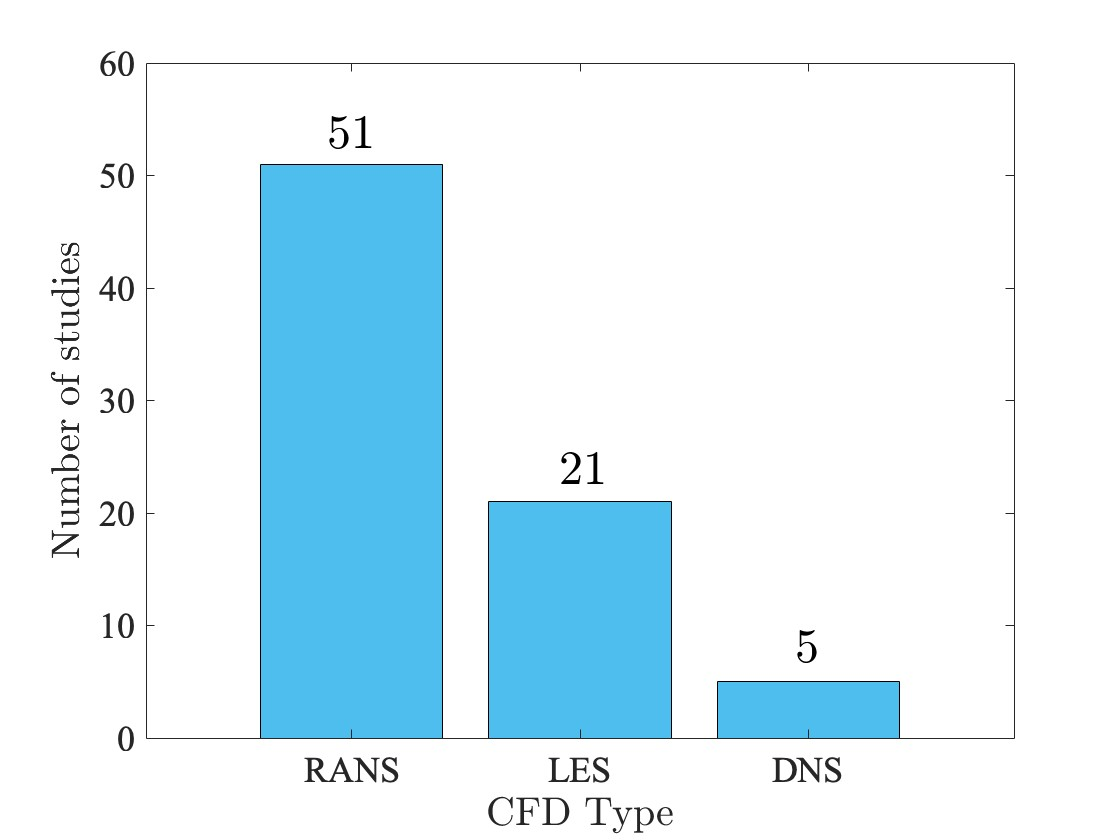
\includegraphics[width=0.5\textwidth]{figures/cfd.jpg}
    \caption{Bar graph depicting the usage of different CFD approaches in indoor airborne transmission studies.}
    \label{fig:cfd}
\end{figure}

While the RANS approach models the entire turbulent kinetic energy spectrum, DNS resolves all the turbulent scales from the largest to the smallest (Kolgomorov) \cite{kolmogorov1941local} scale. DNS has been used to simulate the respiratory jets emanating from people during coughing \cite{rosti2020fluid,diwan2020understanding, chong2021extended} or speech \cite{giri2022colliding, singhal2022virus}, or ventilation flow in a room with an occupant \cite{yerragolam2024effect}. Resolving all the turbulent scales comes at the cost of significant computational resources, making it inaccessible to most researchers. In contrast, More studies recently are resorting to LES for studying airborne transmission in an indoor environment \cite{vuorinen2020modelling,feng2020study,khosronejad2020fluid} as they show more substantial agreement with experimental data when compared to RANS simulations \cite{wu2023numerical}. That is because LES decomposes the flow into two parts: i) Large scales of turbulence that are resolved, and ii) Small scales of turbulence that are unresolved but modelled. Some of the most popular SGS models are the Smaroginsky Lilly model, the Wall Adapting Local Eddy-viscosity (WALE) model, the Vreman model, and the One-equation model. Another approach is Detached Eddy Simulation (DES), where the flow is simulated using LES except within boundary layers and irrotational flow regions, where unsteady RANS simulation is used.

Numerical simulations also have two approaches to handle aerosol transport: Eulerian and Lagrangian. The Eulerian approach considers a fixed domain discretized into a grid, where the fluid properties are spatial fields at each grid point that can vary spatially and temporally within the domain \cite{ferziger2002computational}. The Lagrangian approach tracks the particles instead of the fluid properties, where each particle has its position and velocity \cite{gualtieri2017lagrangian}. Eulerian is advantageous for studying the advection and diffusion of aerosols \cite{pan2022boundary,pan2023predicting}, and is computationally cheaper than Lagrangian particle tracking. However, modelling all the turbulent scales in Eulerian RANS simulations often overestimates dispersion and leads to a well-mixed room condition \cite{ou2022insufficient}. Therefore, Lagrangian simulations provide more detailed information about particle dynamics and evolution \cite{xu2023cfd}, which is ideal for complex and turbulent flows, as is the case here.

In both experimental and numerical approaches of mimicking aerosol transmission in indoor environments, it is observed that often, the respiratory flow from the occupants is generated \cite{zhou2021experimental,romano2015numerical} or modelled  \cite{ren2021numerical,li2023numerical,wu2023numerical} as a constant flow. However, respiratory flow is pulsatile, and the pulsating frequency depends on the respiratory activity \cite{semple1983measurement,kelly2004modeling}. Some have modelled coughs and sneezes like \cite{mirzaie2021covid}, and some have modelled breathing \cite{he2011cfd,shao2021risk}. Speech has not received as much attention yet \cite{giri2022colliding,singhal2022virus}—Additionally, the effect of occupant dynamics on the flow inside an indoor setting. Most studies studying indoor airborne transmission assume perfectly still occupants, while some look into monotonous movements or short sequences. Monotonous movements like walking down an aircraft aisle or inside a patient wardroom \cite{poussou2010flow,wu2023numerical}, while short movements could be opening a door, walking inside a room and then closing the door \cite{saarinen2015large}. Moreover, in settings with more than one occupant, the airflow from the susceptible individuals is ignored \cite{jain2023numerical}.

\section{Conclusions}

In this review, we looked at previous literature from four broad perspectives: (a) transmission of the pathogen, (b) ventilation regime, (c) investigation approach, and (d) setting. These studies were reviewed, and the results were divided into i) Airflow patterns, ii) Droplet dynamics, and iii) Experimental and Numerical approaches. There have been numerous attempts by engineers, scientists, and medical doctors to quantify airborne transmission through experiments, CFD simulations, theoretical models, and epidemiological studies over the last decade. The medical setting has been a primary subject of research in this field. Classroom and office room settings have received some attention among non-medical settings. However, social settings like restaurants haven't received much attention in these studies despite having a high potential for airborne transmission, especially in tropical countries \cite{prata2020temperature}. Since temperature and relative humidity play an essential role in the evolution of pathogen-laden respiratory flow, it has unfortunately remained understated in previous studies. Similarly, the dominant respiratory activities in restaurant settings, such as speaking and breathing, haven't been considered for analysis. Risk assessment is expected in airborne transmission studies and is often performed with the help of theoretical models and quantitative tools. Therefore, the experimental and numerical approaches must be reasonably accurate in replicating the physics, and researchers must be careful about their conclusions. Risk assessment is crucial in determining high-risk zones inside a room, as it helps HVAC engineers and planners develop an optimal ventilation regime. A ventilation regime that either exhausts pathogen-laden aerosol from the high-risk zones or keeps them away from the susceptible occupants' breathing zone. This gives public health organisations precious time to react in the event of an outbreak and implement active measures to contain it.



\section*{Acknowledgements}

This study is part of the Pandemic \& Disaster Preparedness Centre (PDPC) funded frontrunner project “Predicting, measuring and quantifying airborne virus transmission”. The PDPC is a collaboration between the Erasmus Medical Centre, Erasmus University Rotterdam, and the Delft University of Technology. Other participants in this frontrunner project are Erasmus Medical Centre, the University of Utrecht, and the Technical University of Eindhoven, all in the Netherlands.

%% The Appendices part is started with the command \appendix;
%% appendix sections are then done as normal sections



%% If you have bibdatabase file and want bibtex to generate the
%% bibitems, please use
%%
 \bibliographystyle{elsarticle-num-names} 
 \bibliography{cas-refs}

\appendix

%% else use the following coding to input the bibitems directly in the
%% TeX file.

% \begin{thebibliography}{00}

% %% \bibitem{label}
% %% Text of bibliographic item

% \bibitem{}

% \end{thebibliography}
\end{document}
\endinput
%%
%% End of file `elsarticle-template-num.tex'.
